\documentclass{report}
\usepackage[utf8]{inputenc}
\usepackage{amsmath,amssymb,amsthm} % for math stuff
\usepackage{enumitem} % itemsep
\usepackage{graphicx} % for pics
\usepackage[english]{babel}
\usepackage{braket}
\usepackage[export]{adjustbox}
\graphicspath{{./images/}}
\usepackage{caption}
\usepackage{mathtools}
\DeclarePairedDelimiter{\ceil}{\lceil}{\rceil}
\usepackage{geometry}
 \geometry{
 a4paper,
 total={170mm,257mm},
 left=20mm,
 top=20mm,
}
\usepackage{titlepic}
\usepackage{indentfirst}
\usepackage{hyperref}
\hypersetup{
    colorlinks=true,
    linkcolor=blue,
    filecolor=magenta,      
    urlcolor=blue,
}


\title{%
  \huge Quantum Information and Computing\\
  \Large Summer of Science 2020\\}
\author{Mahadevan Subramanian\\
        Roll no. 190260027\\
        Mentor: Thariq Shanavas}
\date{ }
\titlepic{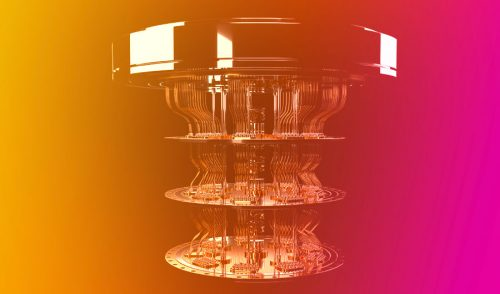
\includegraphics[width=0.7\textwidth]{images/cover2.jpg}}

\begin{document}

\maketitle

\tableofcontents

\chapter{Introduction}

In this chapter I will be discussing some important aspects of computer science and logic which builds up to the quantum computer

\section{Turing Machine}
A Turing machine is an abstract machine, which manipulates symbols on a strip of sufficiently large length according to a table of rules. Given any algorithm a Turing machine can be built to simulate it. According to the strong Church-Turing thesis, a function on the natural numbers can be calculated by an effective method if and only if it is computable by a Turing machine. Essentially it makes claims that all polynomial time computations can be run on a Turing machine since computable generally refers to polynomial time complexity. However it was found out that randomized algorithms can carry out certain efficient computations which cannot be run on a Turing machine clearly violating the strong Church-Turing thesis. This was then modified to being computable on a probabilistic Turing machine.
Now the next step was to actually make a computer that could essentially carry out randomized algorithms and here is where the idea for quantum computation was born

\section{The set of computational problems}
The complete set of computational problems are classified in different sets based on their complexity. PSPACE denotes the set of problems that can be solved using a computer of 'small' size but can do long computations. P denotes the set of problems that can be solved in polynomial time on a deterministic Turing machine an example of which is the shortest path algorithm. NP denotes the set of problems which can be solved in polynomial time by a non deterministic Turing machine essentially requiring a "lucky guess". The set of P lies inside the set NP. NP complete represents a set of NP problems which if solved can essentially extend to the rest of the NP set. PSPACE is believed to include both NP and P within it but it is not properly been proven yet. Factoring is believed to lie in NP but not in NP complete and the interesting thing is that Shor's algorithm can do factoring in polynomial time using a quantum computer. BQP represents problems that can be solved in polynomial time using a quantum computer. We don't yet know the exact extent of this set but it is believed to include P and and also some parts of NP and also problems that lie in PSPACE but not NP.\\\\
%\centering
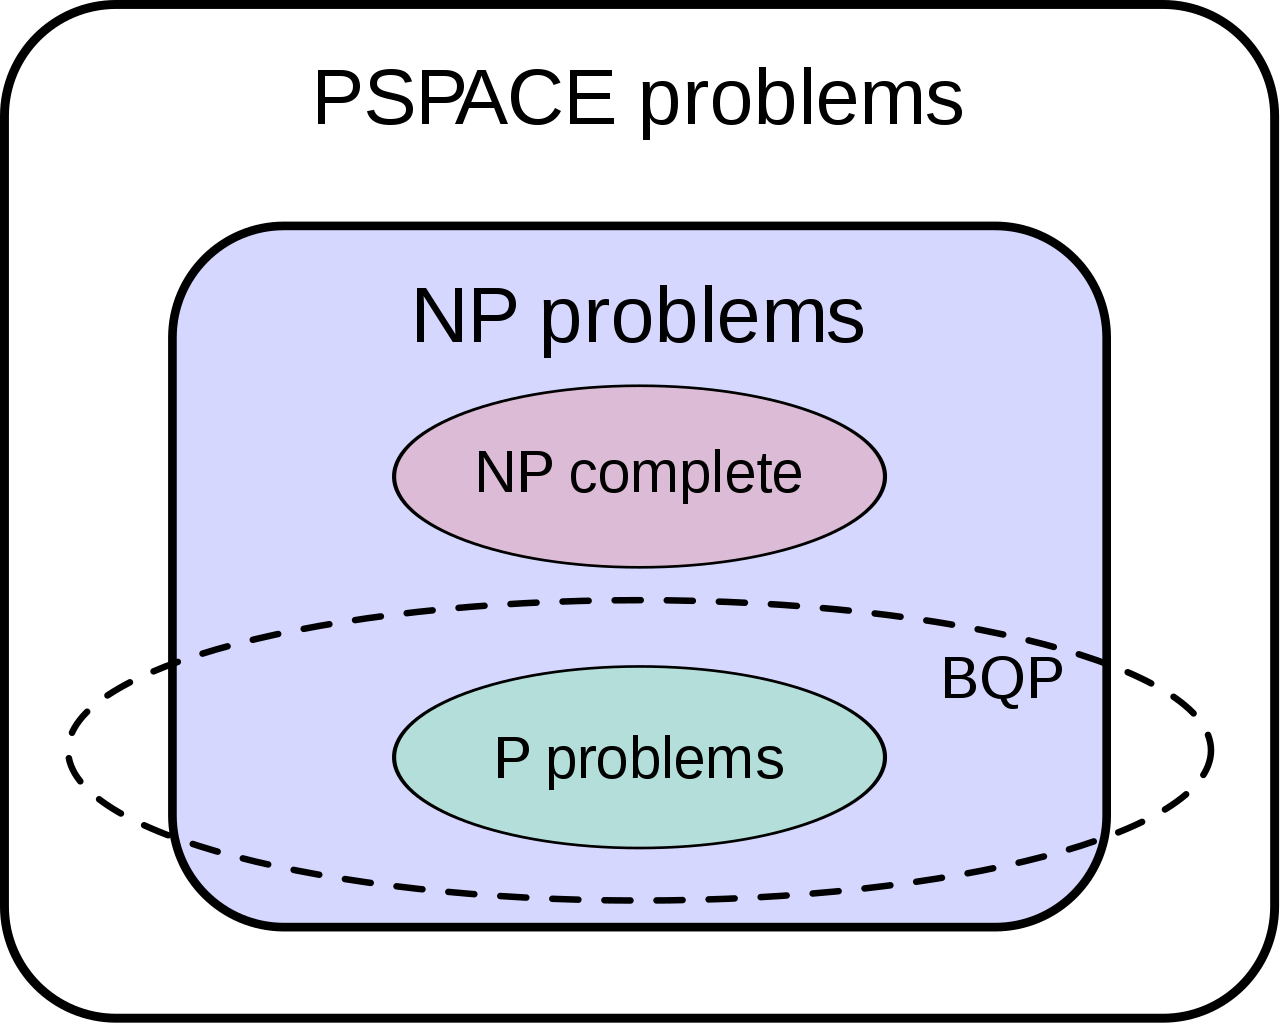
\includegraphics[width = 0.5\textwidth, center]{images/Venn diagram p space.png}
%\captionsetup{labelformat = empty}
%\caption{The set of problems}


\section{Reversible circuits}
An important aspect of quantum computation is that the logical circuits use different kinds of gates and essentially are reversible circuits which work with reversible logic. 
Reversible logic simply means that if we know the output we also know the input hence the input and output have a one one mapping. Right off the bat we know that gates like AND cant be used for this since knowing the output doesn't always tell us enough to know the inputs. 
In a reversible logic circuit the inputs and outputs are equal in number. One can see that in logic circuit like one of an AND gate essentially has less randomness in the output as to the input. 
An important thing to understand is that even though this entropy is in terms of information, it still has an energy price to pay and hence there is a considerable amount of energy consumed in all devices like computers and mobile phones, etc. to repay this entropy loss debt and this is the Von Neumann entropy. In an ideal reversible circuit there is no loss of energy in these terms.\\
An important gate in reversible circuits is the CNOT gate\\
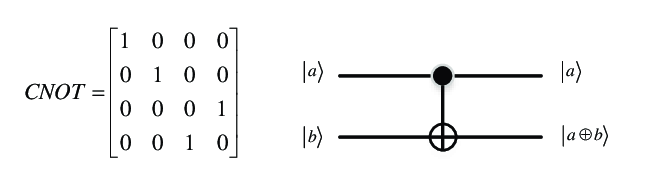
\includegraphics[width = \textwidth]{images/CNOT.png}
Apart from this is the Toffoli gate and the Fredkin gate described in the graphics below.
\begin{figure}[ht]
    \centering
    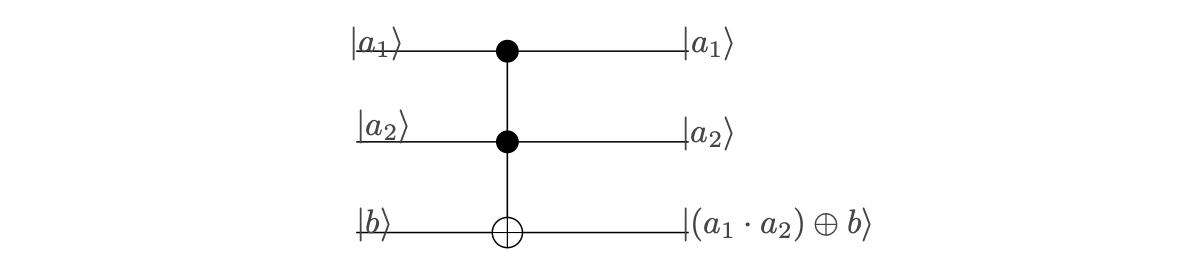
\includegraphics[width = \textwidth]{images/toffoli.png}
    \captionsetup{labelformat = empty}
    \caption{Toffoli gate}
\end{figure}\\
\begin{figure}[ht]
    \centering
    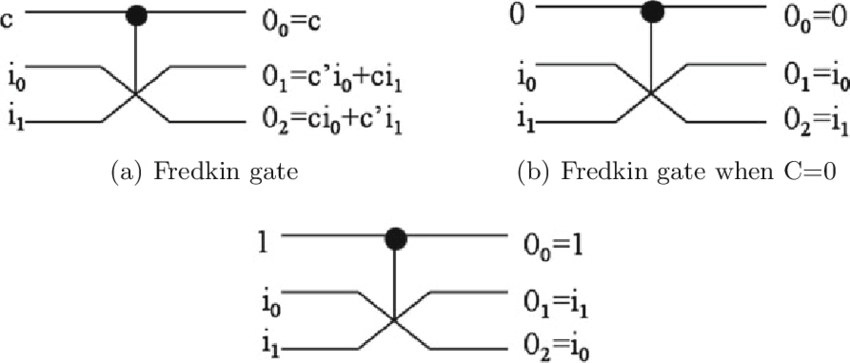
\includegraphics[width = \textwidth]{images/fredkin.png}
    \captionsetup{labelformat = empty}
    \caption{(c) Fredkin gate with c = 1}
\end{figure}\\
An important thing to note is that both these gates are universal i.e. we can reproduce any boolean function purely just using only Toffoli gates and Fredkin gates. As seen below we can implement AND and NOT using Toffoli and Fredkin gates under the following setup\\
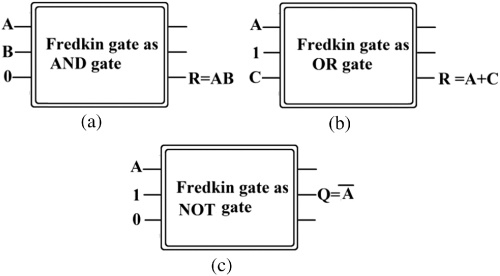
\includegraphics[width = \textwidth]{images/fredkin universal.jpg}\\
It can be proven that using AND gates and NOT gates and FANOUT one can implement all possible boolean functions. (NAND gates are also universal).
All Quantum circuits use reversible logic since we define quantum evolution using unitary transforms which are reversible, hence requiring quantum circuits to also have reversible logic. This is of course broken upon measuring a qubit which will be discussed further ahead.\\
An interesting build of a reversible circuit is the "Billiard ball" model for computing.
We essentially start of by considering two billiard balls A and B which for the sake of simplicity are perfectly elastic and everything in the given environment is ideal.
Let A represent the boolean variable which is true if the ball A is approaching as shown in the figure and is false if it is not present there. Similarly, let B represent the boolean variable which is true if the ball A is approaching as shown in the figure and is false if it is not present there.
One can see that if one were to observe the positions of the balls after some time depending on the values of A and B we will get different scenarios and the presence of a ball at these locations can be represented as the following boolean functions\\
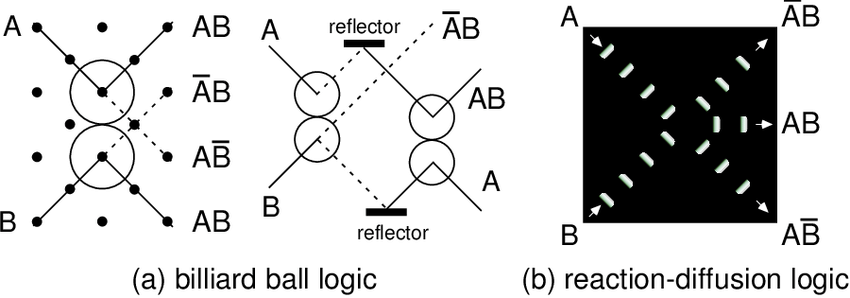
\includegraphics[width = \textwidth]{images/billiard ball.jpg}\\\\
Interestingly there has been no computer built with the billiard ball model since an error in one stage will entirely cause the whole computation to fail and error management wouldn't be that too easy.

\section{Maxwell's Demon}
This is not directly related to computing in the obvious sense but a very interesting thought experiment nonetheless. There was a paradox described by Maxwell in which there is a box filled with gas particles with a middle partition which had a small rolling door. 
A small demon controls this door and only lets particles with a high velocity pass through the door from one side. This act of the demon will decrease entropy despite the demon doing little to no work so this violated the second law of thermodynamics.\\
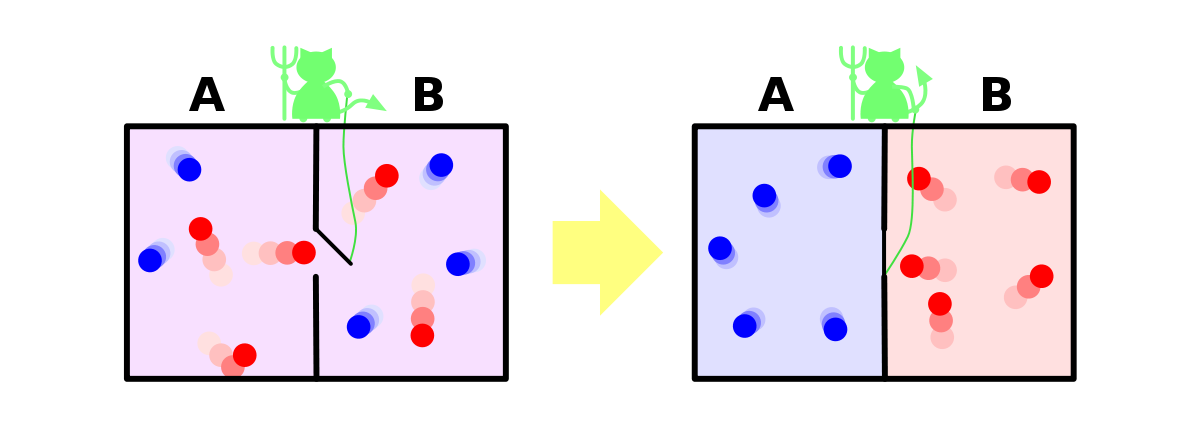
\includegraphics[width = \textwidth]{images/Maxwells demon.png}\\
However an important thing here is that the demon performs measurement over every gas particle as it approaches the door hence he would have to store the information somehow. Since all information storage is finite the demon will eventually reach a point where he would have to erase the information and this actually accounts for the entropy imbalance since erasing information affects entropy by Launder's principle.\\
This is a very interesting link between physics and the idea of information since this concept of entropy related to information plays a very important role as discussed in the previous section regarding reversible circuits.




\chapter{Quantum Mechanics}
In this chapter I will discuss some basic concepts of quantum mechanics which are required for understanding quantum computing
In this report I will be mostly using the bra-ket notation.\\

\section{Postulates of Quantum Mechanics}
The following are the postulates of Quantum mechanics.\\
\textbf{Postulate 1:} The state of a quantum mechanical system is completely specified by the wavefunction $\ket{\psi({\bf r}, t)}$.
\\
\textbf{Postulate 2:} To every observable in classical mechanics, there corresponds a linear, Hermitian operator in quantum mechanics. For example, in coordinate space, the momentum operator ${\hat P}_x$ corresponding to momentum $p_x$ in the $x$ direction for a single particle is $-i \hbar \frac{\partial}{\partial x}$.\\
\textbf{Postulate 3:} In any measurement of the observable associated with operator ${\hat
A}$, the only values that will ever be observed are the eigenvalues $a$ which satisfy ${\hat A} \Psi = a \Psi$. Although measurements must always yield an eigenvalue, the state does not originally have to be in an eigenstate of ${\hat
A}$. An arbitrary state can be expanded in the complete set of eigenvectors of ${\hat A}$ ( ${\hat A} \psi_i = a_i \psi_i$) as $\Psi = \sum_i c_i \psi_i$, where the sum can run to infinity in principle. The probability of observing eigenvalue $a_i$ is given by $c_i^* c_i$.\\
\textbf{Postulate 4:} The average value of the observable corresponding to operator ${\hat{A}}$ is given by 
$\langle\hat{A}\rangle = \dfrac{\bra{\psi}\hat A\ket{\psi}}{\langle\psi|\psi\rangle}$ \\
\textbf{Postulate 5:} The wavefunction evolves in time according to the time-dependent Schrödinger equation
\begin{equation*}
\displaystyle i\hbar {\frac {\partial }{\partial t}}|\psi (t)\rangle ={\hat {H}}|\psi (t)\rangle\end{equation*}
H represents the Hamiltonian of the state and $\ket{\psi}$ represents the state of the system.\\
\textbf{Postulate 6:} The total wavefunction must be anti symmetric with respect to the interchange of all coordinates of one fermion with those of another. Electronic spin must be included in this set of coordinates. The Pauli exclusion principle is a direct result of this anti symmetry principle.
\\


\section{Qubits}

\subsection{What is a Qubit}
A qubit is a form of information which essentially represents the wave function of a two level quantum mechanical system. These two levels are represented as $\ket{0}$ and $\ket{1}$ and the state is written as a linear combination of these two i.e. $\ket{\psi} = \alpha\ket{0} + \beta\ket{1}$. Here $\alpha,\beta\in\mathbb{C}$ with constraint $|\alpha|^2 + |\beta|^2 = 1$ for normalization purposes.\\
Measurement of a qubit causes it to "collapse" onto one of the states $\ket{0}$ or $\ket{1}$ and the probability for it to be measured as $\ket{0}$ is $|\alpha|^2$ and for $\ket{1}$ it is $|\beta|^2$. For representation we represent these kets as two dimensional column vectors.\\
$\ket{0} = \begin{bmatrix} 1\\0\end{bmatrix}$ and $\ket{1} = \begin{bmatrix}0\\1\end{bmatrix}$. So essentially $\ket{\psi} = \begin{bmatrix} \alpha\\\beta\end{bmatrix}$\\
Qubits are meant to represent information but handling them is not as easy as handling classical bits due to the fact that they lose their information once measured and also they cannot be cloned. However there are many interesting things that can be done with qubits due to the nature of Quantum mechanics and most of their advantages stem from quantum entanglement.\\
An interesting analogue of qubits are dreams. Say you just had a dream while you slept and on waking up you remember the details of your dream but you wouldn't be able to communicate the exact details of your dream since it is present by itself in a somewhat vague state. So once you try to describe it to someone you would essentially forget the original information and you dream collapses to the description you had given. Not exactly a perfect analogue but an interesting one nonetheless.

\subsection{Bloch Sphere}
A method used for visualization of qubits is the Bloch sphere representation. Since all qubits are written as $\alpha\ket{0} + \beta\ket{1}$ with $|\alpha|^2 + |\beta|^2 = 1$. 
Since $\alpha$ and $\beta$ are complex numbers it is possible to represent each qubit with three real numbers. An important point to understand here is that global phase change over a qubit doesn't affect it. 
Hence the qubits $\alpha\ket{0} + \beta\ket{1}$ and $e^{\iota\theta}(\alpha\ket{0} + \beta\ket{1})$ are the same since there is no way to differentiate between them.\\
$\ket{\psi} = \alpha\ket{0} + \beta\ket{1}$ with $|\alpha|^2 + |\beta|^2 = 1$ can be written as\\
\begin{equation}\ket{\psi} = \cos(\theta/2)\ket{0} + e^{\iota\phi}\sin(\theta/2)\ket{1}\end{equation}
Note that since global phase is ignored we can assume $\alpha$ to take on real values.
If we take a sphere centered at origin and assume $\ket{0}$ to represent $\ket{+z}$ and $\ket{1}$ to represent $\ket{-z}$ we get that the angle $\theta$ from eq 2.1 actually is the polar angle of the vector which connects the origin to the point which actually represents this qubit and the angle $\phi$ represents the azimuthal angle.\\
Using this we get $\ket{+x} = \dfrac{\ket{0} + \ket{1}}{2}$ and $\ket{-x} = \dfrac{\ket{0} - \ket{1}}{2}$.
Also $\ket{+y} = \dfrac{\ket{0} + \iota\ket{1}}{2}$ and $\ket{-y} = \dfrac{\ket{0} - \iota\ket{1}}{2}$.\\
We often write $\ket{+x}$ as $\ket{+}$ and $\ket{-x}$ as $\ket{-}$.
We can define certain operations over qubits which actually rotate the qubit about a certain axis by a certain angle. These are called single qubit gates.\\
\begin{figure}[ht]
    \centering
    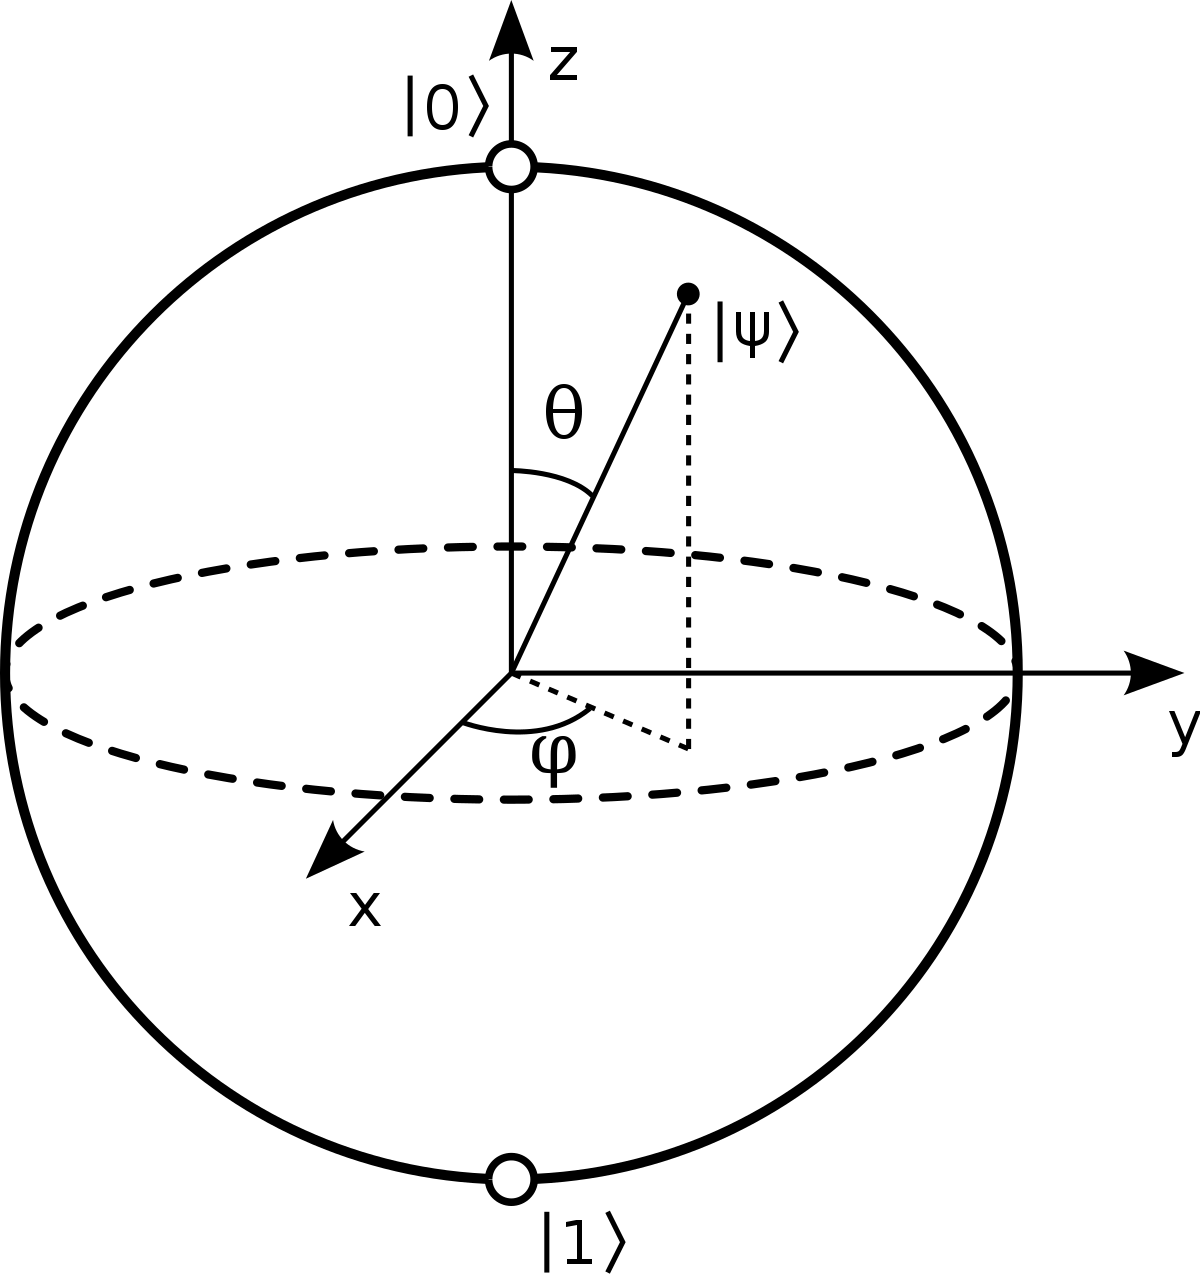
\includegraphics[scale = 0.16]{images/Bloch sphere.png}
    %\captionsetup{labelformat = empty}
    \caption{Bloch Sphere}
    \label{fig:my_label}
\end{figure}\\
Some important ones are the Pauli sigma matrices $\sigma_x$, $\sigma_y$, $\sigma_z$. Their eigenvalues are +1 and -1 and their eigenvectors are the corresponding axes like for $\sigma_x$ the eigenvectors are $\ket{+x}$ with eigenvalue 1 and $\ket{-x}$ with eigenvalue -1
They essentially rotate by $\pi$ about their respective axes. When represented in the $\ket{0}$, $\ket{1}$ basis these are the Pauli sigma matrices:
$\sigma_x = \begin{bmatrix}0 & 1\\1 & 0\end{bmatrix}$, $\sigma_y = \begin{bmatrix}0 & -\iota\\\iota & 0\end{bmatrix}$, $\sigma_z = \begin{bmatrix}1 & 0\\0 & -1\end{bmatrix}$.\\
For performing rotation we define the rotation operators $R_x(\theta) = e^{-\iota\frac{\theta}{2}\sigma_x}$, $R_y(\theta) =  e^{-\iota\frac{\theta}{2}\sigma_y}$, $R_z(\theta) =  e^{-\iota\frac{\theta}{2}\sigma_z}$ where each of these respectively rotates by an angle of theta about the respective axes.
Using this we can prove that rotation about a unit vector $\hat{n}$ by an angle $\theta$ can be written as $R_{\hat{n}}(\theta) = e^{-\iota\frac{\theta}{2}\hat{n}.\sigma}$. Here $\hat{n}.\sigma = n_x\sigma_x + n_x\sigma_y + n_x\sigma_z$.\\
When used in quantum circuits, $\sigma_x, \sigma_y, \sigma_z$ are written as $X, Y, Z$ respectively and are used as gates.
Also a very frequently used gate the Hadamard gate is written as $H = \dfrac{1}{\sqrt{2}}\begin{bmatrix}1 & 1\\1 & -1\end{bmatrix}$ and essentially performs a rotation about the vector $(\frac{1}{\sqrt{2}},0,\frac{1}{\sqrt{2}})$ by an angle $\pi$. Note that I am ignoring any global phase changes since they are irrelevant.

\subsection{No-Cloning theorem}
The no-cloning theorem states that it is impossible to create an identical copy of an arbitrary unknown quantum state. Essentially one cannot simply clone a qubit. The proof of this is as follows:\\
Let there be two slots A and B in a quantum computer. A is the data slot which has an unknown state $\ket{\psi}$ and B is the target slot where we wish to copy the given state so it is initially in a known state $\ket{s}$.\\
Let us define a unitary evolution $U$ such that applying $U$ to this given state makes a clone of the data slot to the target slot. Current state is,
\begin{equation}\ket{\psi}\otimes\ket{s}\end{equation}
On applying unitary transform $U$,
$$U(\ket{\psi}\otimes\ket{s}) = \ket{\psi}\otimes\ket{\psi}$$
Suppose this cloning procedure were to work for two particular pure states $\ket{\psi}$ and $\ket{\phi}$, We have
\begin{equation}U(\ket{\psi}\otimes\ket{s}) = \ket{\psi}\otimes\ket{\psi}\end{equation}
\begin{equation}U(\ket{\phi}\otimes\ket{s}) = \ket{\phi}\otimes\ket{\phi}\end{equation}
On taking the inner product of these two equations we get
\begin{equation}\langle\psi|\phi\rangle = (\langle\psi|\phi\rangle)^2\end{equation}
On solving this equation, we get that either $\ket{\psi} = \ket{\phi}$ or $\ket{\psi}$ and $\ket{\phi}$ are orthogonal hence we cannot have a unitary cloning operation which can clone non orthogonal states simultaneously. 

\section{Quantum measurement}
Quite possibly one of the most perplexing aspects of quantum mechanics has to be measurement.
\subsection{Projective Measurements}
When measurement is done of a state over a certain basis the wavefunction collapses onto one of the orthonormal states which belong to that basis.
We can define there to be certain measurement operator $M_m$ where the index m denotes which state it will collapse to. With this we get\\
\begin{equation*}p(m) = \bra{\psi}{M_m}^{\dagger}M_m\ket{\psi}\end{equation*}
\begin{equation*}\ket{\psi^{'}} = \dfrac{M_m\ket{\psi}}{\sqrt{\bra{\psi}{M_m}^{\dagger}M_m\ket{\psi}}}\end{equation*}
Here $\ket{\psi^{'}}$ represents the state after measurement and $p_m$ is the probability for it to collapse onto that state.
Since these measurements only give us a final result over an orthonormal basis it is not possible to differentiate between non orthogonal states.\\
Also these measurement operators must follow the completeness property that $\sum_m{{M_m}^{\dagger}M_m} = I$.

\subsection{Heisenberg's uncertainty principle}
According to the Heisenberg's uncertainty principle, one cannot measure two non commuting operators to full accuracy. Its proof goes like this.\\
Let there be two Hermitian operators $A$ and $B$ and there is a state $\ket{\psi}$\\
Let $\bra{\psi}AB\ket{\psi} = x + {\iota}y$ where $x,y \in \mathbb{R}$. Since $A$ and $B$ are Hermitian we have $\bra{\psi}BA\ket{\psi} = x - {\iota}y$.
Therefore\\
\begin{equation}|\bra{\psi}[A,B]\ket{\psi}|^2 + |\bra{\psi}\{A,B\}\ket{\psi}|^2 = 4|\bra{\psi}AB\ket{\psi}|^2\end{equation}
By Cauchy-Shwarz inequality we have
\begin{equation}|\bra{\psi}AB\ket{\psi}|^2 \leq \bra{\psi}A^2\ket{\psi}\bra{\psi}B^2\ket{\psi}\end{equation}
on combining 2.7 with eq 2.6 we get
\begin{equation}|\bra{\psi}[A,B]\ket{\psi}|^2 \leq 4\bra{\psi}A^2\ket{\psi}\bra{\psi}B^2\ket{\psi}\end{equation}
Lets take two observable $C$ and $D$, Let $A = C - \langle{C}\rangle$ and $B = D - \langle{D}\rangle$. On substituting this to eq 2.8 we get
\begin{equation}\Delta(C)\Delta(D) \geq \dfrac{|\bra{\psi}[C,D]\ket{\psi}|}{2}\end{equation}
And this is the Heisenberg uncertainty relation
Here $\Delta(C)$ represents the standard deviation of the values of $C$. In its exactness the Heisenberg uncertainty relation states that if we have prepared a large number of identical states $\ket{\psi}$, and we were to measure the observables $C$ and $D$ over this system we would get multiple values for them however their standard deviations will follow this inequality. Hence we mustn't think of these as accuracy limitations but as uncertainty in the value we wish to observe.

\subsection{POVM Measurements}
Projective measurements follow in a way that once the state is measured it remains the same hence doing the same measurement will yield the exact same state with 100\% probability. 
However there are forms of measurement which cannot be repeated to give the same state. For example if we were to measure the position of a photon using a silvered screen we end up destroying the photon.\\
POVM stands for positive operator valued measure. We define $E_m = {M_m}^{\dagger}M_m$ where $M_m$ are the measurement operators. So we have $\sum_m{E_m} = I$ by the completeness property. We call $E_m$ as the POVM elements. We also have $p(m) = \bra{\psi}E_m\ket{\psi}$
Projective measurements are essentially a case of POVM where we have $M_m = \sqrt{E_m}$.\\
An interesting thing to note is that we can use POVM elements to try to differentiate between non orthogonal states. Say we are given one of the two qubits $\ket{\psi_1} = \ket{0}$ and $\ket{\psi_2} = \dfrac{\ket{0} + \ket{1}}{\sqrt{2}}$. Using just projective measurements we would not be able to conclude with complete certainty which state we have been given however say we define the following POVM elements
$$E_1 = \dfrac{\sqrt{2}}{1 + \sqrt{2}}\ket{1}\bra{1}$$
$$E_2 = \dfrac{\sqrt{2}}{1 + \sqrt{2}}(\ket{0} - \ket{1})(\bra{0} - \bra{1})$$
$$E_3 = I - E_1 - E_2$$
Clearly this follows completeness property. One can see that if we get $E_1$ we can be sure that we received $\ket{\psi_2}$ and if we get $E_2$ we can be sure that we received $\ket{\psi_1}$. However we cant make any conclusion if we obtain $E_3$. However we can safely conclude that our assumptions wont be wrong.
This can be extended to any number of qubits say $m$ by using $m + 1$ POVM elements by smartly choosing each $E_i$ according to what makes each $\ket{\psi_i}$ different from the rest. 



\section{Density matrices}
Density matrices are an important extension of a quantum state. An important property of a density matrix is that it stores the complete information of the state. We represent it by $\rho$. Suppose we have an ensemble of states $\{p_i, \ket{\psi_i}\}$ where $p_i$ is the probability of getting $\ket{\psi_i}$, then we represent density matrix as
$$\rho = \sum_{i}p_i\ket{\psi_i}\bra{\psi_i}$$
When describing evolution of density matrix for some unitary evolution $U$ over $\ket{\psi}$ we get the following ($\rho^{'}$ represents evolved density matrix)
$$\rho^{'} = \sum_{i}p_{i}U\ket{\psi_i}\bra{\psi_i}U^{\dagger} = U{\rho}U^{\dagger}$$
An important concept in density matrices is the distinction between pure states and mixed states. For a pure state we know its exact $\ket{\psi}$ hence the density matrix is simply $\rho = \ket{\psi}\bra{\psi}$. 
Otherwise, $\rho$ is in a mixed state, it is said to be a mixture of the different pure states in the ensemble for $\rho$.
An obvious fact is that $tr(\rho) = 1$ since the wavefunction has to be normalised. For a pure state we get $tr({\rho}^2) = 1$ but for a mixed state $tr({\rho}^2) < 1$.\\
For the case where the state is prepared with some density matrix $\rho_i$ with probability $p_i$ we can denote the density matrix as $\sum_{i}p_{i}\rho_{i}$. To prove this lets say that $\rho_i$ arises from some ensemble $\{p_{ij},\ket{\psi_{ij}}\}$ hence probability for state $\ket{\psi_{ij}}$ is $p_{i}p_{ij}$. So we get
$$\rho = \sum_{ij}p_{i}p_{ij}\ket{\psi_{ij}}\bra{\psi_{ij}} = \sum_{i}p_{i}\rho_{i}$$
An interesting property of the density operator is that different states can generate the same density operator. Suppose we have two sets $\ket{\tilde{\psi_i}}$ and $\ket{\tilde{\phi_j}}$. Let $\ket{\tilde{\psi_i}} = \sum_{j}u_{ij}\ket{\tilde{\phi_j}}$ for some unitary $u_{ij}$. Then we have
\begin{equation}\sum_{i}\ket{\tilde{\psi_i}}\bra{\tilde{\psi_i}} = \sum_{ijk}u_{ij}{u^{*}}_{ik}\ket{\tilde{\phi_j}}\bra{\tilde{\phi_j}}\end{equation}
\begin{equation}\sum_{i}\ket{\tilde{\psi_i}}\bra{\tilde{\psi_i}} = \sum_{jk}\left(\sum_{i}{u_{ki}}^{\dagger}u_{ij}\right)\ket{\tilde{\phi_j}}\bra{\tilde{\phi_j}}\end{equation}
\begin{equation}\sum_{i}\ket{\tilde{\psi_i}}\bra{\tilde{\psi_i}} = \sum_{jk}\delta_{kj}\ket{\tilde{\phi_j}}\bra{\tilde{\phi_j}}\end{equation}
\begin{equation}\sum_{i}\ket{\tilde{\psi_i}}\bra{\tilde{\psi_i}} = \sum_{j}\ket{\tilde{\phi_j}}\bra{\tilde{\phi_j}}\end{equation}
We can clearly see that these two construct the same density operator as per the relation assumed. For the converse if we start with eq 2.13 we can retrace back to get the above assumed relation.\\
Another important thing is the representation of mixed states on the Bloch sphere. For pure states the state is represented by a point on the Bloch sphere. Interestingly for mixed states, the state is represented by a point inside the sphere. Let there be a state $\ket{\psi}$ then we know that $\rho = \dfrac{I + \vec{r}.\sigma}{2}$. This can be proved very easily since $\rho$ is hermitian.\\
One can also see that for a mixed state $|\vec{r}| < 1$. This vector $\vec{r}$ is called the Bloch vector of $\rho$.

\subsection{Partial Trace and Reduced density operator}
Suppose we have a density operator $\rho^{AB}$ which describes two systems $A$ and $B$. The reduced density operator for system A is defined as the following
$$\rho^{A} = tr_{B}(\rho^{AB})$$
$tr_{B}$ is just the trace over the system B. Partial trace is defined as this
$$tr_{B}(\ket{a_1}\bra{a_2} \otimes \ket{b_1}\bra{b_2}) = \ket{a_1}\bra{a_2}tr(\ket{b_1}\bra{b_2})$$
Since its a composite system we write $\rho^{AB}$ as a tensor product. The reduced density operator is a very useful tool. Lets assume we have the following state $\ket{\psi} = \dfrac{\ket{00} + \ket{11}}{\sqrt{2}}$. This happens to be one of the bell pairs. So we have
\begin{equation}\rho = \dfrac{\ket{00}\bra{00} + \ket{11}\bra{00} + \ket{00}\bra{11} + \ket{11}\bra{11}}{2}\end{equation}
For reduced density operator for the first qubit we have
\begin{equation}\rho^1 = tr_{2}(\rho)\end{equation}
\begin{equation}\rho^1 = \dfrac{\ket{0}\bra{0} + \ket{1}\bra{1}}{2} = \dfrac{I}{2}\end{equation}
So we can see that the Bloch vector for $\rho^1$ is actually zero hence it must be a mixed state which is pretty weird since we happen to know $\ket{\psi}$ completely. Interestingly we get the same result for all the bell pairs.\\
An interesting property of the partial trace is that it is a unique function for creating a map from operators in $AB$ to operators in $A$. Also reduced density operator explains why quantum teleportation makes sense but more on that later.

\subsection{Schmidt Decomposition}
According to the Schmidt decomposition theorem, suppose $\ket{\psi}$ is a pure state of a composite system, $AB$. Then there exist orthonormal states $\ket{i_A}$ for system $A$, and orthonormal states $\ket{i_B}$ of system $B$ such that
$$\ket{\psi} = \sum_{i}\lambda_{i}\ket{i_A}\ket{i_B}$$
Where $\lambda_i$ are non-negative real numbers satisfying $\sum_{i}{\lambda_i}^2 = 1$ known as Schmidt coefficients. This is a very strong result since we don't need $A$ and $B$ to even be of the same dimension. Also as a result of this we get $\rho^{A} = \sum_{i}{\lambda_{i}}^2\ket{i_A}\bra{i_A}$ and $\rho^{B} = \sum_{i}{\lambda_{i}}^2\ket{i_B}\bra{i_B}$ so essentially we get that $\rho^{A}$ and $\rho^{B}$ have the same eigen values. The following is the proof for this theorem.\\
We know that for an operator $O_A$ in $A$ and some suitable $\rho^A$
\begin{equation}\langle\psi|(O_A \otimes I)\psi\rangle = tr({O_{A}}\rho^A)
\end{equation}
This is a consequence of the decomposition so our aim is to prove this.
There exists some orthonormal basis say $\ket{i_A}$ such that
\begin{equation}\rho^{A}\ket{i_A} = p_{i}\ket{i_A}\end{equation}
Lets now define the state in this basis along with some arbitrary basis in B $\ket{\phi_{i}}$
\begin{equation}\ket{\psi} = \sum_{ij}c_{ij}\ket{i_A}\ket{\phi_{i}} = \sum_{i}\ket{i_A}\left(\sum_{j}c_{ij}\ket{i_B}\right)\end{equation}
if we set $\sum_{j}c_{ij}\ket{\phi_{i}} = c_{i}\ket{i_B}$ for some unit vector $\ket{i_B}$ and a positive $c_i$. Now we have
\begin{equation}\ket{\psi} = \sum_{i}c_{i}\ket{i_A}\ket{i_B}\end{equation}
We know that
\begin{equation}tr({O_{A}}\rho_1) = \sum_{i}\bra{i_A}{O_{A}}\rho_{1}i_{A}\rangle = \sum_{i}p_{i}\bra{i_A}{O_{A}}i_{A}\rangle\end{equation}
\begin{equation}\langle\psi|(O_A \otimes I)\psi\rangle = \sum_{j}{c_i}^{*}{c_j}\bra{i_A}O_{A}j_{A}\rangle\langle{i_B}|{j_B}\rangle\end{equation}
$\langle{i_B}|{j_B}\rangle$ disappears for $i \neq j$ so we actually get RHS in eq 2.22 equal to RHS in eq 2.21. So we get $|c_i|^2 = p_i$ and if we take $c_i$ as positive then we get $c_i = \sqrt{p_i}$. Now if we repeat this process by starting with some operator $O_B$ in $B$ we get that their density matrices have the same eigen values hence proving our theorem.
Interestingly we didn't need to assume that $A$ and $B$ are of the same dimension in all of this. So we get
\begin{equation}\langle\psi|(I \otimes O_B)\psi\rangle = tr({O_{B}}\rho^B)
\end{equation}
When it comes down to it we can break down a two system state into the form stated in the theorem and that actually gives rise to some very interesting symmetries. For example in the state $\ket{\psi} = \dfrac{\ket{00} + \ket{01} + \ket{11}}{\sqrt{3}}$ using Schmidt decomposition we get that $tr((\rho^A)^2)$ and $tr((\rho^B)^2)$ both come out to be as $7/9$. The symmetry here is not very obvious but essentially involves breaking it down in a way that the density operators for the two systems have the same eigen values.
Also this cannot be extended to three systems since cross terms cannot be avoided there.\\
Another important thing which can be done with this is purification. It essentially works this way. We are given a density matrix $\rho^A$ of a system $A$. We can now introduce another system $R$ and define a pure system $\ket{AR}$ in both these systems such that $\rho^{A} = tr_{R}(\ket{AR}\bra{AR})$. This is known as purification and allows us to associate a pure state to a mixed state. If we define $\ket{AR}$ like this
$$\ket{AR} = \sum_{i}\sqrt{p_i}\ket{i_A}\ket{i_R}$$
Using this we get
\begin{equation}tr_{R}(\ket{AR}\bra{AR}) = \sum_{ij}\sqrt{p_{i}p_{j}}\ket{i_A}\bra{j_A}tr(\ket{i_R}\bra{j_R})\end{equation}
\begin{equation}tr_{R}(\ket{AR}\bra{AR}) = \sum_{ij}\sqrt{p_{i}p_{j}}\ket{i_A}\bra{j_A}\delta{ij}\end{equation}
\begin{equation}tr_{R}(\ket{AR}\bra{AR}) = \sum_{i}p_{i}\ket{i_A}\bra{i_A} = \rho^{A}\end{equation}
One must note that using some $U_{R}\ket{R}$ instead of $\ket{R}$ where $U_{R}$ is a unitary evolution in $R$ also gives a purification

\section{EPR and the Bell inequality}
This would quite possibly be one of the most debated topics in Quantum mechanics. In their 1935 paper Einstein, Polensky and Rosen offered an argument to prove that the current Quantum theory is incomplete. 
Their idea was later refined by David Bohm and today is mainly presented in this form. Suppose we prepare a two qubit state like this, $\ket{\psi} = \dfrac{\ket{01} - \ket{10}}{\sqrt{2}}$. If we measure the first qubit and we get $\ket{1}$ we reach the conclusion that the second qubit would have to become $\ket{0}$ and vice-versa however this violates the idea of local realism which had been assumed to be true.\\ 
Later in Bell's 1971 paper Bell assumed a local deterministic world along with the hidden variables theory and reached an inequality which could be checked experimentally. He concluded in this paper that it is not possible for a hidden variable theory to support local determinism. I wont go over the exact math in that paper however later his inequality gave rise to the CSHS inequality.\\
The experimental setup is something like this, two people Alice and Bob (better get used to these names as they come up quite often) are given one of the qubits from the previously mentioned $\ket{\psi}$. They have a choice to measure along different vectors in the way that Alice can either measure along $\vec{q}$ and $\vec{r}$ and get values $Q$ or $R$. Similarly Bob can measure along $\vec{s}$ and $\vec{t}$ and get values $S$ or $T$. Note that all of $Q,R,S,T$ take either +1 or -1 as a value.\\
According to Bell's inequality we get
$$E(QS) + E(RS) + E(RT) - E(QT) \leq 2$$
But here's the issue, nature doesn't follow this inequality. Various experiments have been performed and it turns out that this inequality isn't completely true and the actual bound comes out to be $2\sqrt{2}$. This is mainly because the math involved in deriving this was actually done without considering any quantum mechanics and the commutation relations between observables. This was refined in the Tsirelon's inequality which essentially sets the higher bound as $2\sqrt{2}$.\\
It goes like this, we take $Q = \vec{q}.\vec{\sigma}$, $R = \vec{r}.\vec{\sigma}$, $S = \vec{s}.\vec{\sigma}$, $T = \vec{t}.\vec{\sigma}$.
We can prove the following equation
\begin{equation}(Q \otimes S + R \otimes S + R \otimes T - Q \otimes T)^2 = 4I + [Q,R] \otimes [S, T]\end{equation}
from here on taking average value on both sides and using the inequality from eq. 2.8 we get the following equation
\begin{equation}\langle{Q \otimes S}\rangle + \langle{R \otimes S}\rangle + \langle{R \otimes T}\rangle - \langle{Q \otimes T}\rangle \leq 2\sqrt{2}\end{equation}
This is the Tsirelon's inequality.

%\chapter*{Updated Plan of Action}
%\addcontentsline{toc}{chapter}{Updated Plan of Action}
%The updated plan of action is as follows\\
%\textbf{Week 4:} Quantum circuits, Quantum teleportation, Kraus operators\\
%\textbf{Week 5:} Quantum Search algorithms, Quantum Fourier transform, Shor's algorithm\\
%\textbf{Week 6:} Superdense coding, Deutsch algorithm\\
%\textbf{Week 7:} Doing stuff on IBM Quantum experience\\
%\textbf{Week 8:} Overflows and completing the report


\chapter{Quantum Circuits}
In this chapter I will be discussing the various quantum gates and building quantum circuits

\section{Quantum Gates}
All quantum gates are essentially a unitary evolution which acts on a state. For single qubits an important thing to observe about these are that they are all unitary operations and can be described as a global phase multiplication along with rotations about the $x, y, z$ axes.\\
Let there be some unitary evolution $U$ acting on a single qubit state. We can prove that all unitary evolutions can be defined in the following way
\begin{equation}
U = e^{i\alpha}R_x(\beta)R_y(\gamma)R_z(\delta)
\end{equation}
Here $R_x, R_y, R_z$ are the rotation operators as defined in the section 2.2.2 in the previous chapter. The phase term is irrelevant when multiplied to a single qubit but ahead we will see that it can be used over a multiple qubit system to actually change it.
The following are some important quantum gates which we will be seeing quite often\\
\begin{figure}[ht]
    \centering
    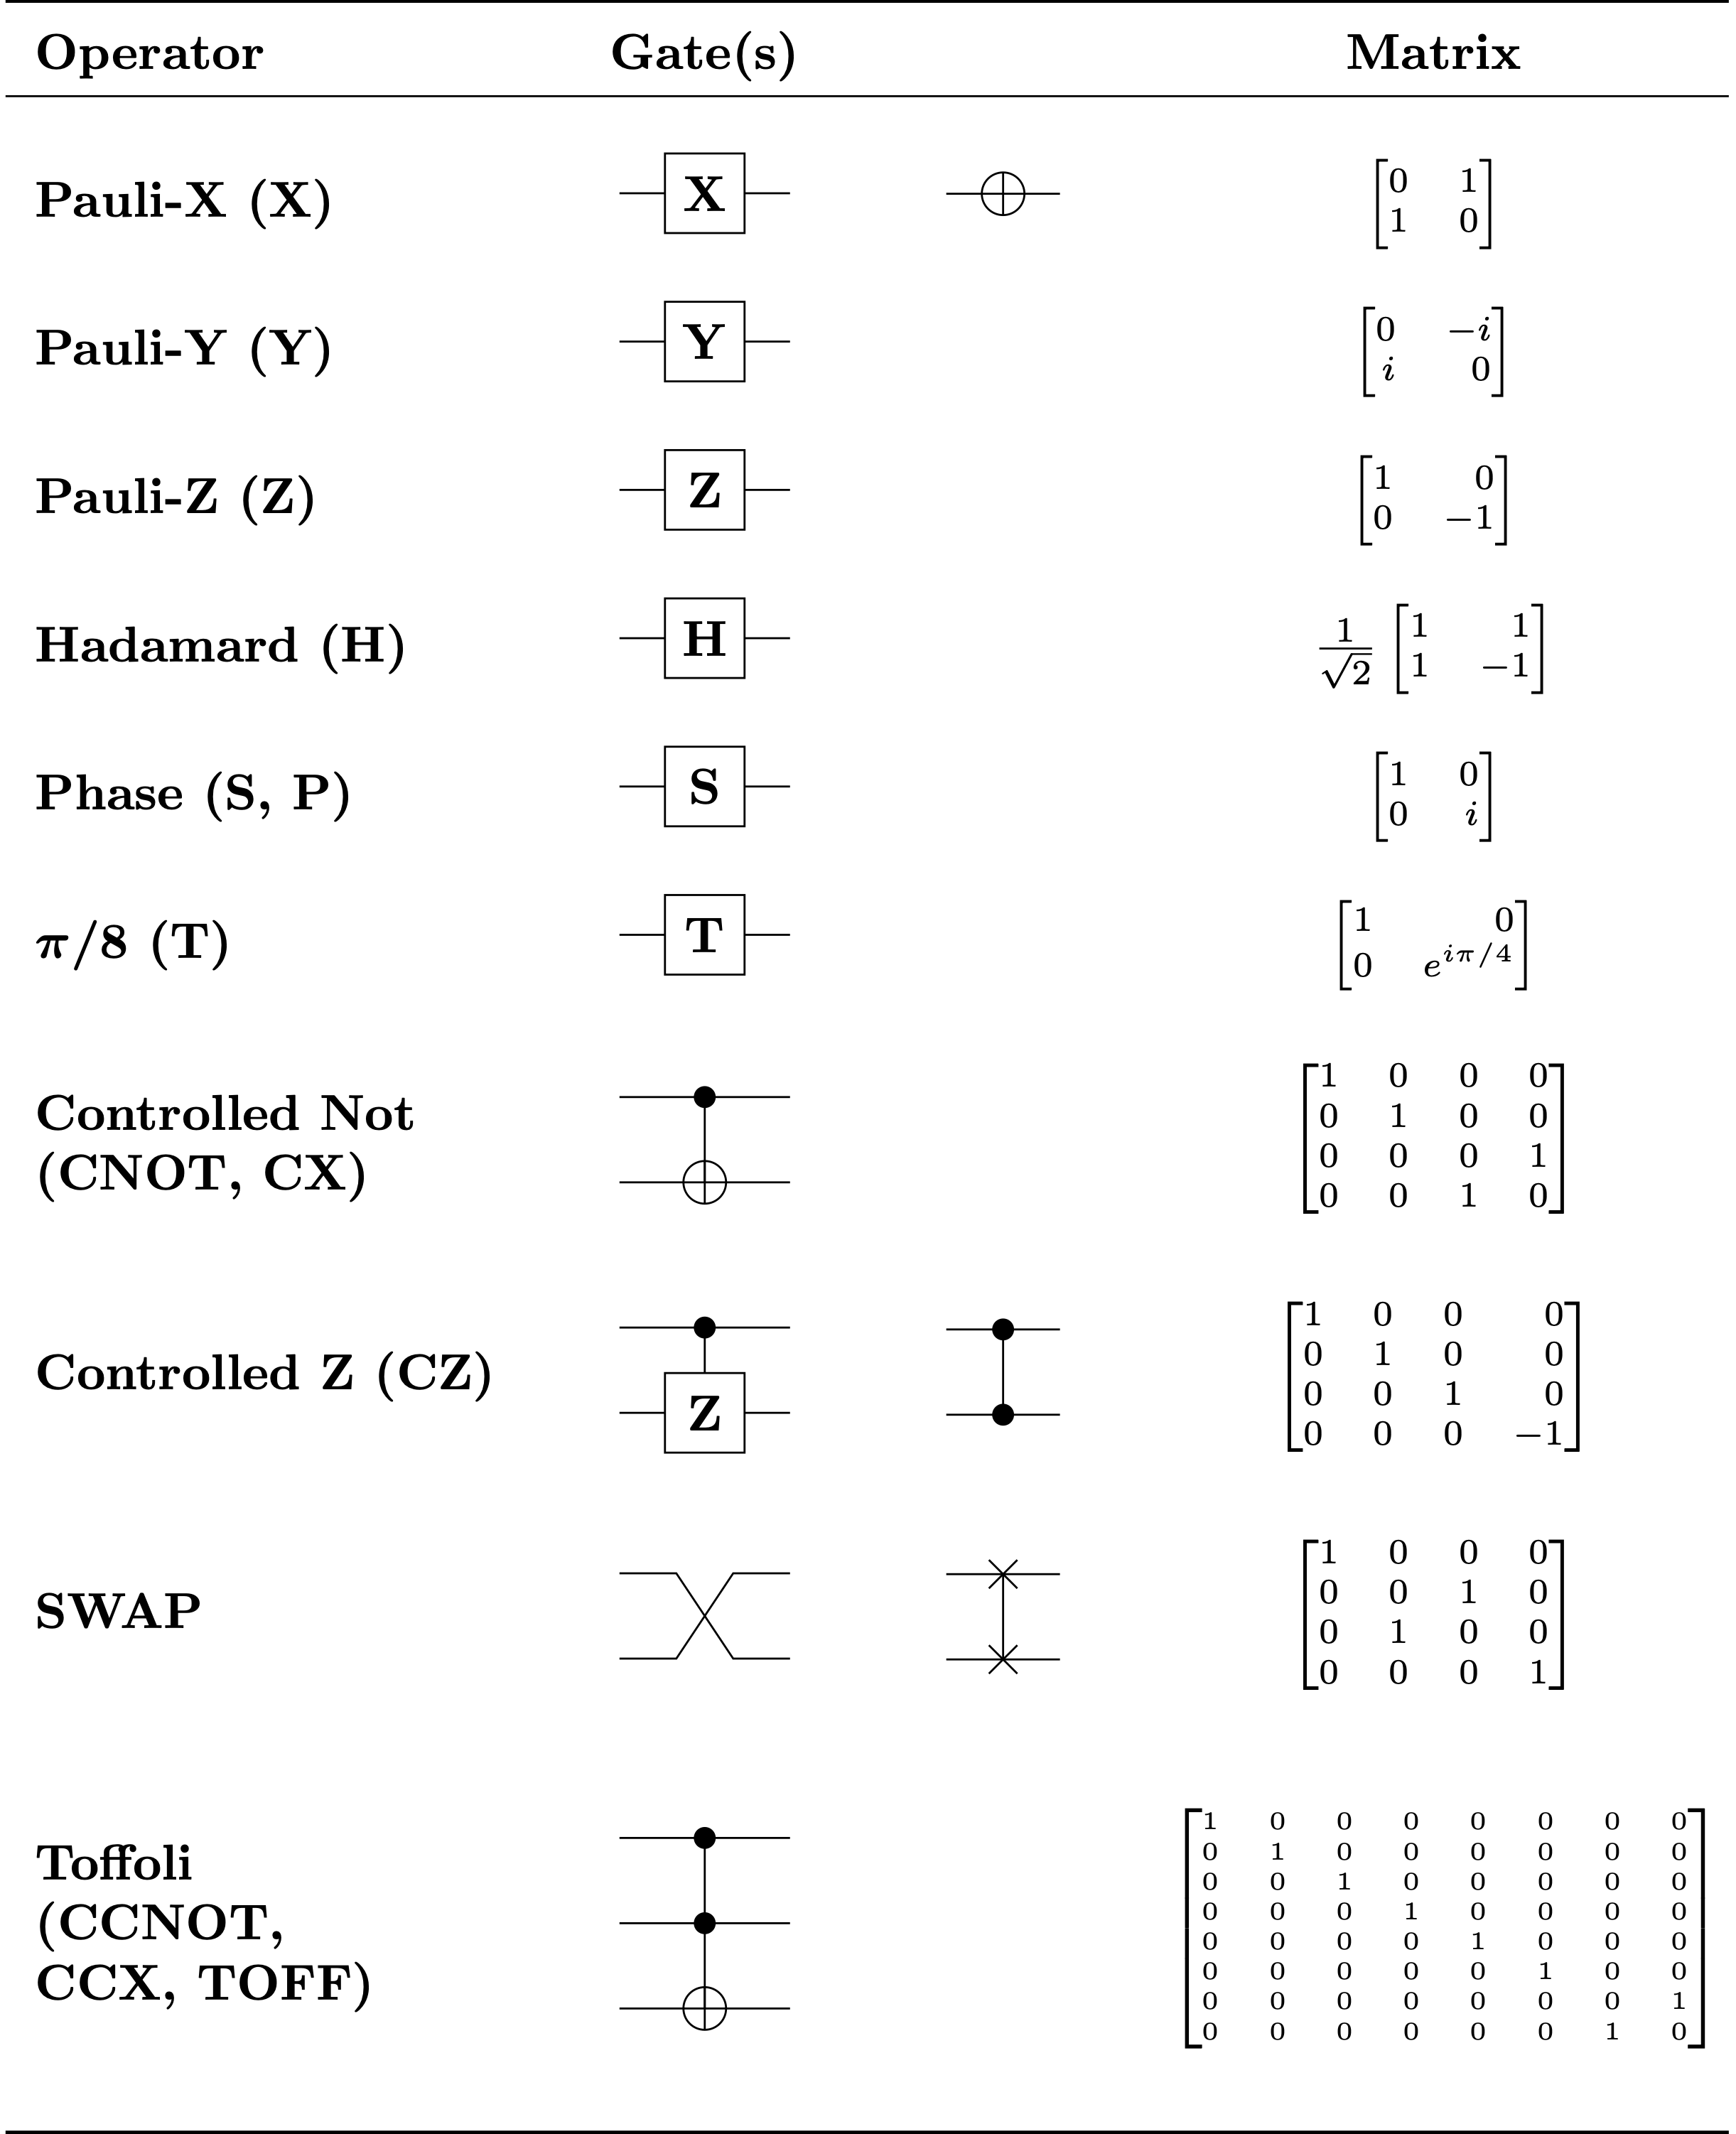
\includegraphics[width = 0.5\textwidth]{images/Quantum_Logic_Gates.png}
    \caption{Quantum Gates}
    %\label{fig:my_label}
\end{figure}
On a side note the $T$ gate which is called the $\pi/8$ gate actually causes a rotation of $pi/4$ and affects the global phase by $\pi/8$ hence the name is actually quite deceiving hence we will be referring to it as the $T$ gate only.\\
This formulation of eq 3.1 can also be extended like this
\begin{equation}
U = e^{i\alpha}R_{\hat{n}}(\beta)R_{\hat{m}}(\gamma)R_{\hat{n}}(\delta)
\end{equation}
Here $\hat{n}$ and $\hat{m}$ are two non parallel unit vectors about which the rotations are occurring and $\alpha, \beta, \gamma, \delta$ are chosen appropriately for the unitary operation.\\
Another interesting way of writing the unitary operator is $U = AXBXC$ where $ABC = I$. This can be easily verified by putting $A = R_z(\beta)R_y(\gamma/2)$, $B = R_y(-\gamma/2)R_z(-(\delta + \beta)/2)$ and $C = R_z((\delta - \beta)/2)$ and using eq, 3.2 with $\hat{n} = \hat{z}$ and $\hat{m} = \hat{y}$. Clearly $ABC = I$ and using the identity $XR_y(\theta)X = R_y(-\theta)$ and $XR_z(\theta)X = R_z(-\theta)$ we get $U = AXBXC$.\\
Some other identities using single qubits are 
$$HXH = Z, HYH = -Y, HZH = X$$

\subsection{Controlled gates}
Controlled gates which is controlled by $n$ qubits ($\ket{x_1,x_2,....x_n}$) and causes a unitary evolution $U$ over $k$ qubits (state $\ket{\psi}$) is described by the following gate $C^n(U)$ in this equation
\begin{equation}C^n(U)\ket{x_1,x_2,....x_n}\ket{\psi} = \ket{x_1,x_2,....x_n}U^{x1x2...xn}\ket{\psi}\end{equation}
Put simply it applies the operation $U$ over $\ket{\psi}$ when all of $x_1,x_2,....x_n$ are 1.\\
One can see that the controlled not ($CNOT$) described in the figure above is a controlled gate. Using this gate entangles the two qubits it acts on. We can also describe a controlled unitary operator using one qubit for control using the $U = AXBXC$ method where $ABC = I$ in the following manner.
\begin{figure}[ht]
    \centering
    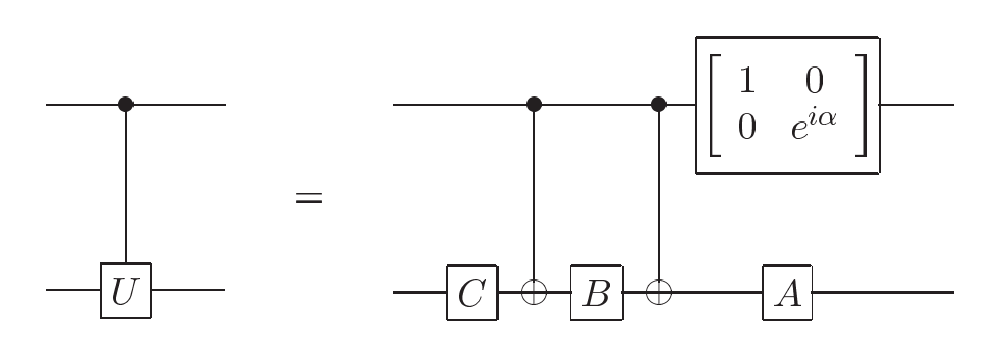
\includegraphics[width = 0.6\textwidth]{images/unitary.png}
    \caption{A $C^1(U)$ gate}
    %\label{fig:my_label}
\end{figure}
The Toffoli gate is a not controlled by two qubits. It can be constructed using $CNOT, H, T, T^{\dagger}$ as shown in fig. 3.3\\
\begin{figure}[ht]
    \centering
    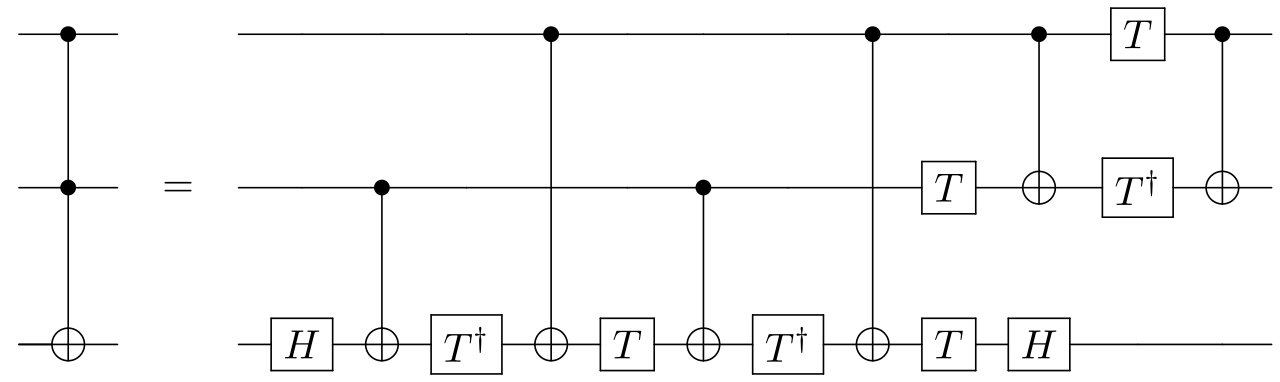
\includegraphics[width = \textwidth]{images/toffoli construction.png}
    \caption{Toffoli gate construction}
    %\label{fig:my_label}
\end{figure}\\
If we are to make a $C^2(U)$ gate we can construct it using $CNOT$ and $V$ gates where $V^2 = U$ and $V$ is unitary. The ciruit would be something like this (refer fig. 3.4).
\begin{figure}[ht]
    \centering
    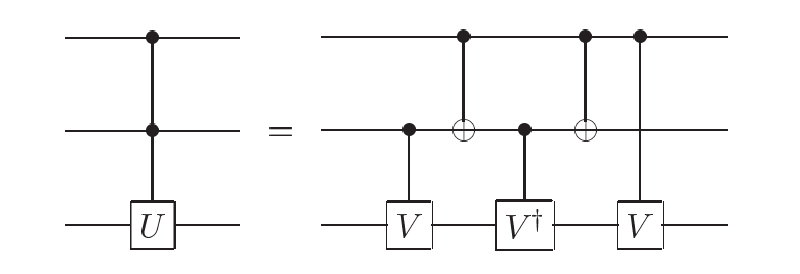
\includegraphics[width = 0.6\textwidth]{images/unitary 2 control.png}
    \caption{A $C^2(U)$ gate}
    %\label{fig:my_label}
\end{figure}
If we wish to execute a Toffoli gate we can put $V = \dfrac{(1 - \iota)(I + \iota{X})}{2}$\\
For constructing a fredkin gate using toffoli gates is quite simple. It can even be constructed using one toffoli and two CNOTs as shown here.\\
\begin{figure}[ht]
\centering
\begin{minipage}{.5\textwidth}
\centering
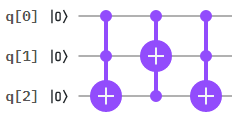
\includegraphics[width=.5\linewidth]{images/fredkin with toffoli.png}
\captionof{figure}{Fredkin using toffoli}
\label{fig:test1}
\end{minipage}%
\begin{minipage}{.5\textwidth}
\centering
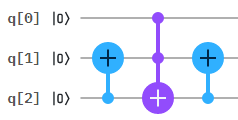
\includegraphics[width=.5\linewidth]{images/fredkin with cnot.png}
\captionof{figure}{Fredkin using CNOT and toffoli}
\label{fig:test2}
\end{minipage}
\end{figure}\\
However an interesting thing about the fredkin gate is that it can be constructed completely with only five two qubit gates. In fig. 3.6 replacing the toffoli by a construction like that of fig. 3.4 we get fig. 3.7 where $V^2 = X$ and $V$ is unitary.\\
\begin{figure}[ht]
\centering
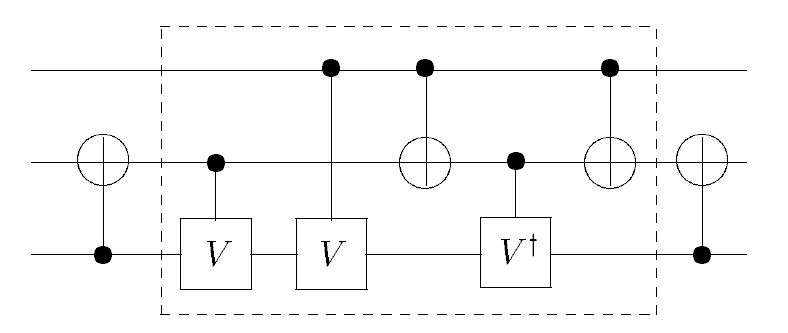
\includegraphics[width = 0.6\textwidth]{images/fredkin with 5 gates.png}
\caption{Fredkin with 5 two qubit gates}
\end{figure}
The two $CNOTs$ in the right end commute and so we can combine the last $CNOT$ with the controlled $V^{\dagger}$ and similarly combine the first $CNOT$ and the controlled $V$. This yields us five two qubit gates.\\
Say we want to construct a $C^5(U)$ gate we can do so in a simple method using ancillary or work qubits along with some toffoli gates.\\
\begin{figure}[ht]
\centering
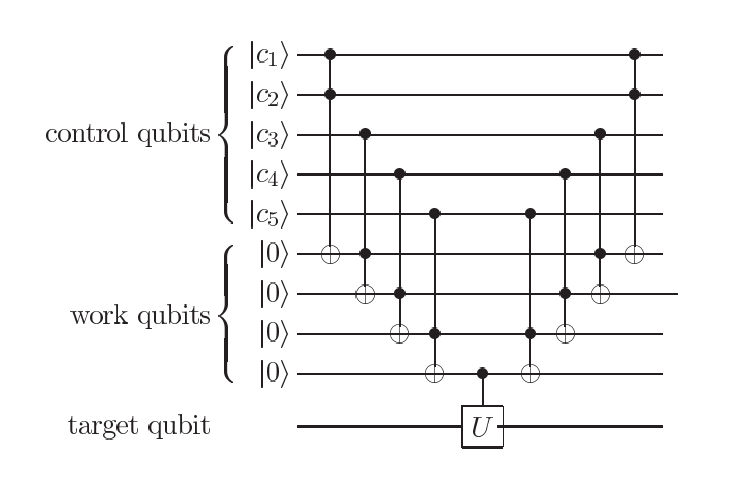
\includegraphics[width = 0.5\textwidth]{images/c5u.png}
\caption{$C^5(U)$ with work qubits}
\end{figure}\\
This can easily be extended to $C^n(U)$ however the issue is that there is a lot of work qubits involved. Say we want to execute $C^n(Z)$.
We can actually solve this quite easily using the method described in fig. 3.4 for executing this. So we can see that if we use $C^{n-1}(X)$ with it acting on the $n^th$ qubit controlled by the first $(n-1)$ qubits, followed by controlled $\sqrt{Z}^{\dagger}$ which acts on the target qubit controlled by $n^th$ qubit. 
This is followed by another $C^{n-1}(X)$  acting on the $n^th$ controlled by the first $(n-1)$ bits and after this we have a controlled $\sqrt{Z}$ gate which acts on the target qubit controlled by the $n^th$ qubit. This is followed by a $C^{n-1}(\sqrt{Z})$ gate which acts on the target qubit and is controlled by the first $n-1$ qubits. We can now break this gate down recursively following the previous procedure and using controlled $\sqrt[\leftroot{-1}\uproot{1}4]{Z}$ gates and go on till we only have gates which can be controlled by a single qubit.\\
\begin{figure}[ht]
\centering
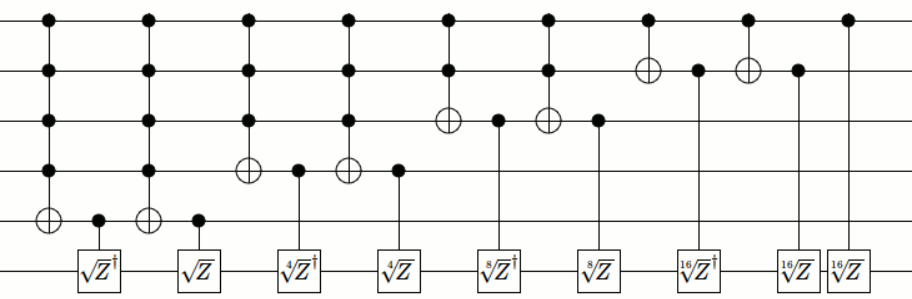
\includegraphics[width = \textwidth]{images/iterative.png}
\caption{Iteratively executing a $C^5(Z)$}
\end{figure}\\
Note that even though we are using multiple control not gates they too can be broken down in a similar process so we can construct the whole thing just using toffolis and CNOTs and two qubit gates. However the circuit complexity has gone in $O(n^2)$ in comparison to the work qubit method.\\
Another thing about controlled gates is that when a certain control qubit has a white dot on it, it implies that the $NOT$ of that qubit is being used in control. Refer fig. 3.10.
\begin{figure}[ht]
\centering
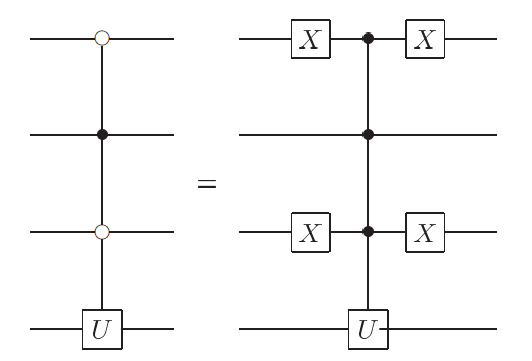
\includegraphics[width = 0.3\textwidth]{images/white dots.png}
\caption{Controlled gates with white dots}
\end{figure}\\

\subsection{Measurement in circuits and Quantum Teleportation}
\begin{figure}[ht]
\centering
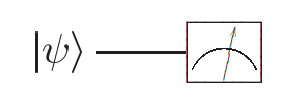
\includegraphics[width = 0.2\textwidth]{images/measurement.png}
\caption{Measurement in Quantum circuits}
\end{figure}
Measurement always has only two possibilities $\ket{0}$ and $\ket{1}$ however one can measure on a different basis by simply multiplying the appropriate operator to the state before measurement. For example if we wish to measure in the $\ket{+}$ and $\ket{-}$ basis then one has to apply the Hadamard gate before measurement.\\
An important equality in measurement is that if we have $C^1(U)$ and we apply measurement before the gate on the controlling qubit it is the same as measuring the qubit after applying the gate.\\
An important application of quantum computing arises with using measurement and that is quantum teleportation. In Quantum teleportation we essentially transport an unknown state from one qubit to another.\\
So we have the original state $\ket{\psi}$ and two other qubits initialized at $\ket{B_{00}}$ which is the EPR pair $\dfrac{\ket{00} + \ket{11}}{\sqrt{2}}$ and they follow the given circuit (fig. 3.11)\\
\begin{figure}[ht]
\centering
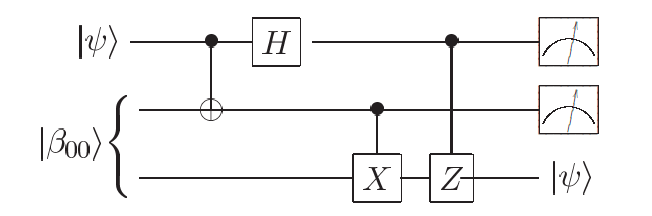
\includegraphics[width = 0.6\textwidth]{images/teleportation.png}
\caption{Quantum Teleportation}
\end{figure}\\
To think of the teleportation in terms of the receiver and sender we can think of it this way. Alice and Bob have an EPR pair with them with each having one of the qubits. Alice now makes the qubit with state $\ket{\psi} = \alpha\ket{0} + \beta\ket{1}$ interact with her qubit from the EPR pair and then measures both the qubits and based on her results Bob applies the appropriate transformations over his qubit and will then obtain the state $\ket{\psi}$ on his qubit.\\
Initially the state of the system is $\ket{\psi_0} = \ket{\psi}\ket{\beta_{00}}$. We can see that after the $CNOT$ and $H$ gates the state of the system is $\ket{\psi_1} = \dfrac{1}{2}\big[\alpha(\ket{0} + \ket{1})(\ket{00} + \ket{11}) + \beta(\ket{0} - \ket{1})(\ket{01} + \ket{10})\big]$ this can be rearranged into the following
$$\ket{\psi_1} = \dfrac{1}{2}\big[\ket{00}(\alpha\ket{0} + \beta\ket{1}) + \ket{01}(\alpha\ket{0} + \beta\ket{1}) + \ket{10}(\alpha\ket{0} - \beta\ket{1}) + \ket{11}(\alpha\ket{1} - \beta\ket{0})\big]$$
Hence on measuring the first two qubits and applying appropriate transformation to the third qubit will make it into the original state $\ket{\psi}$.
Note that since Bob requires the result of Alice's measurement to obtain the original state and that is possible only via a classical channel of communication there is no violation of relativity occurring.\\
Now if we were to calculate the density operator of the state $\ket{\psi_1}$ we see that its equal to the following\\
$\rho = \dfrac{1}{4}\big[\ket{00}\bra{00}(\alpha\ket{0} + \beta\ket{1})(\alpha^*\bra{0} + \beta^*\bra{1}) + \ket{01}\bra{01}(\alpha\ket{1} + \beta\ket{0})(\alpha^*\bra{1} + \beta^*\bra{0}) + \ket{10}\bra{10}(\alpha\ket{0} - \beta\ket{1})(\alpha^*\bra{0} - \beta^*\bra{1}) + \ket{10}\bra{10}(\alpha\ket{1} - \beta\ket{0})(\alpha^*\bra{1} - \beta^*\bra{0})\big]$\\
The reduced density operator for Bob's state can be calculated using partial trace.
$$\rho_B = \dfrac{2(|\alpha|^2 + |\beta|^2)\ket{0}\bra{0} + 2(|\alpha|^2 + |\beta|^2)\ket{1}\bra{1}}{4} = \dfrac{I}{2}$$
Clearly this contains no information about $\ket{\psi}$ hence without the measurement and communication of the result Bob has no information regarding $\ket{\psi}$ at all hence this doesn't violate relativity at all.


\section{Universality in Quantum Computing}
We know that using $NAND$ gates alone one can implement all boolean functions. Similarly we can also implement any arbitrary unitary evolution using just CNOT, Hadamard, Phase and $pi/8$ gates upto an arbitrary level of accuracy. It is important to understand that one cannot represent every unitary evolution since they exist over a continuous set of variables hence could require an infinite number of these gates to execute.\\

\subsection{Two level unitary operators}
One can perform all unitary evolutions using just CNOT gates and single qubit gates. To understand this we must first see that we can represent every unitary evolution as a product of some number of two level unitary matrices.\\
A two level unitary matrix is a which affects only two or fewer of the components of the vector it acts on. A $d$ dimensional unitary matrix can be written as a product of at most $d(d-1)/2$ two level unitary matrices. The steps in finding this unitary decomposition is to keep making the diagonal elements of $U$ equal to 1 and make the rest of the row and column zero and at each stage we will get a two level unitary evolution to multiply. repeat till we don't end up with a two level unitary matrix.\\
Now if we want to execute a two level unitary operation we can do so using single qubit gates and $CNOT$ gates. So first of all let the two level unitary operation be some $U$. This acts only on two binary sequences say $\ket{g_1}$ and $\ket{g_m}$ and these are connected by the gray code $\ket{g_2}, \ket{g_3},....\ket{g_{m-1}}$. \\
A gray code is a sequence where each term differs from the last by just a single bit. Lets say the $\ket{g_{m-1}}$ and $\ket{g_m}$ differ in their $j^th$ bit, then we have to construct a controlled operation such that it acts the unitary $\Tilde{U}$ on the $j^th$ qubit and is controlled by the rest of the cubits. Here $\Tilde{U}$ is the sub matrix of $U$ which makes it differ from an identity matrix. However this must be applied after we interchange the $\ket{g_1}$ state with $\ket{g_{m-1}}$\\
Here is an example. Suppose we wish to execute the unitary $U$ which is the following.
$$U = \begin{bmatrix}
      a & 0 & 0 & 0 & 0 & 0 & 0 & c\\
      0 & 1 & 0 & 0 & 0 & 0 & 0 & 0\\
      0 & 0 & 1 & 0 & 0 & 0 & 0 & 0\\
      0 & 0 & 0 & 1 & 0 & 0 & 0 & 0\\
      0 & 0 & 0 & 0 & 1 & 0 & 0 & 0\\
      0 & 0 & 0 & 0 & 0 & 1 & 0 & 0\\
      0 & 0 & 0 & 0 & 0 & 0 & 1 & 0\\
      b & 0 & 0 & 0 & 0 & 0 & 0 & d\\
      \end{bmatrix}$$
Clearly $\Tilde{U} =\begin{bmatrix}a & c\\b & d\end{bmatrix}$ and the two states $U$ affects is $\ket{000}$ and $\ket{111}$. The gray code sequence between them is $\ket{000}\xrightarrow{}\ket{001}\xrightarrow{}\ket{011}\xrightarrow{}\ket{111}$. Here the last two terms differ in their first qubit and we must exchange the state $\ket{000}$ with $\ket{011}$. We can see that the following circuit in fig. 3.13 does this.
\begin{figure}[ht]
\centering
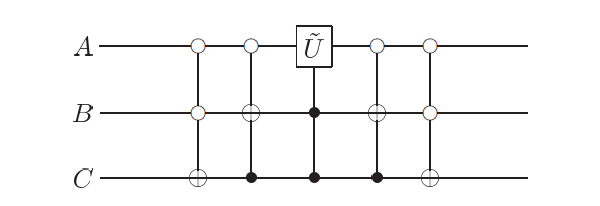
\includegraphics[width = 0.6\textwidth]{images/two level unitary.png}
\caption{Executing the circuit for the operation $U$}
\end{figure}\\
Its trivial to see that this circuit can be broken into $CNOTs$ and single qubit gates using methods described previously. For a two level unitary evolution we can see that it takes complexity of $O(n^2)$ on breaking down into $CNOTs$ and single qubit gates. If we were to extend this to an arbitrary unitary evolution we can see that it will become $O(n^{2}2^{2n})$ since an arbitrary unitary evolution can be represented as a product of $O((2^n)^2)$ since the operator is $2^n$ dimensional and the number of two level matrices required is in $n^2$ complexity.\\

\subsection{Approximating Unitary operators}
Now here's the thing. Notice how we so freely used any arbitrary single qubit gate? Well we often just cannot come up with any arbitrary unitary operation over a single qubit so easily.\\
We will now define a quantity $E(U,V)$ where $U$ and $V$ are unitary operators of the same state space.
\begin{equation}E(U,V) = max||(U - V)\ket{\psi}||\end{equation}
The max represents the maximum over all possible $\ket{\psi}$ in the state space. Suppose a quantum system starts in the state $\ket{\psi}$, and we perform either the unitary operation $U$, or the unitary operation $V$ . Following this, we perform a measurement. Let $M$ be a POVM element associated with the measurement, and let $P_U$ (or $P_V$) be the probability of obtaining the corresponding measurement outcome if the operation $U$ (or $V$) was performed. We then have
\begin{equation}|P_U - P_V| = |\bra{\psi}U^{\dagger}MU\ket{\psi} - \bra{\psi}V^{\dagger}MV\ket{\psi}|\end{equation}
If we substitute $\ket{\Delta} = (U - V)\ket{\psi}$ we get the following from Cauchy-Schwarz inequality
\begin{equation}|P_U - P_V| = |\bra{\psi}U^{\dagger}M\ket{\Delta} + \bra{\Delta}MV\ket{\psi}|\end{equation}
\begin{equation}|P_U - P_V| \leq ||\ket{\Delta}|| + ||\ket{\Delta}||\end{equation}
\begin{equation}|P_U - P_V| \leq 2E(U,V)\end{equation}
Hence if $E(U,V)$ is small, the measurement results of $U$ and $V$ will also be very close. Note that if we use sequenced gates, the error value will add up linearly and so wouldn't actually cause big problems
\begin{equation}E(U_{2}U_{1} - V_{2}V_{1}) = ||(U_{2}U_{1} - V_{2}V_{1})\ket{\psi}||\end{equation}
\begin{equation}E(U_{2}U_{1} - V_{2}V_{1}) = ||(U_{2}U_{1} - V_{2}U_{1})\ket{\psi} + (V_{2}U_{1} - V_{2}V_{1})\ket{\psi}||\end{equation}
\begin{equation}E(U_{2}U_{1} - V_{2}V_{1}) = ||(U_{2}U_{1} - V_{2}U_{1})\ket{\psi} + (V_{2}U_{1} - V_{2}V_{1})\ket{\psi}||\end{equation}
Using triangle inequality we get
\begin{equation}E(U_{2}U_{1} - V_{2}V_{1}) \leq ||(U_{2} - V_{2})U_{1}\ket{\psi}|| + ||U_{1} - V_{1})V_{2}\ket{\psi}||\end{equation}
\begin{equation}E(U_{2}U_{1} - V_{2}V_{1}) \leq E(U_2,V_2) + E(U_1,V_1)\end{equation}
This can be extended to any number of operations using induction.\\
Consider the operations $T$ and $HTH$. $T$ gives a rotation about $Z$ axis by an angle of $pi/4$. $HTH$ gives a rotation about $X$ axis by an angle of $pi/4$. Combining these both we get
\begin{equation}
\exp(-\iota\dfrac{\pi}{8}Z)\exp(-\iota\dfrac{\pi}{8}X) = \Big[\cos\left(\dfrac{\pi}{8}\right)I - {\iota}\sin\left(\dfrac{\pi}{8}\right)Z\Big]\Big[\cos\left(\dfrac{\pi}{8}\right)I - {\iota}\sin\left(\dfrac{\pi}{8}\right)X\Big]
\end{equation}
\begin{equation}
\exp(-\iota\dfrac{\pi}{8}Z)\exp(-\iota\dfrac{\pi}{8}X) = {\cos}^2\left(\dfrac{\pi}{8}\right)I - \iota\Big[\cos\left(\dfrac{\pi}{8}\right)(X + Z) + \sin\left(\dfrac{\pi}{8}\right)Y\Big]\sin\left(\dfrac{\pi}{8}\right)
\end{equation}
As one can see this obtains us a rotation by an $\theta$  such that $\cos\left(\dfrac{\theta}{2}\right) = {\cos}^2\left(\dfrac{\pi}{8}\right)$ about the vector $\vec{n} = \left(\cos\dfrac{\pi}{8},\sin\dfrac{\pi}{8},\cos\dfrac{\pi}{8}\right)$. We can see that this $\theta$ is an irrational multiple of $2\pi$. Hence suppose we wish to make $R_{\vec{n}}(\alpha)$ for some arbitrary $\alpha$ we can replicate to an arbitrary accuracy using repeated iteration $R_{\vec{n}}(\theta)$\\
Lets say we wish to have it to some accuracy $\delta$ and $N$ is an integer larger than $2\pi/\delta$. Lets define a sequence $\theta_k = (k\theta)$mod $2\pi$. From pigeonhole principle we can see that there exists distinct $j,k \in{1,2,.....N}$ such that $|\theta_j - \theta_k| \leq 2\pi/N < \delta$ hence we can use $\theta_{l(j-k)}$ to attain any value in $[0, 2\pi)$ with accuracy of $\delta$.\\
Now we can see that $HR_{\vec{n}}(\theta)H = R_{\vec{m}}(\theta)$ where $\vec{m} = \left(\cos\dfrac{\pi}{8},-\sin\dfrac{\pi}{8},\cos\dfrac{\pi}{8}\right)$. Now if we recall eq. 3.2, we can see that all unitary operators can be represented as the following subject to a certain level of accuracy.
\begin{equation}
U = e^{i\alpha}{R_{\vec{n}}(\theta)}^{n_1}H{R_{\vec{n}}(\theta)}^{n_2}H{R_{\vec{n}}(\theta)}^{n_3}
\end{equation}
Now here is the important question. How efficient is this approach? Say we have $m$ gate circuit we wish to replicate to closeness of $\epsilon$ (we define this closeness as $E(U,V) < \epsilon$). This will give us a $\Omega(m2^{(m/\epsilon)})$ which is not really good however with the $\theta_k$ approach we can see that the range of angles gets filled up fairly uniformly so we can consider a complexity of some $\Theta(m^2/\epsilon)$. This gives us a fairly good approach however it can get even better. According to the Solovay-Kitaev theorem one can achieve a complexity of $O(mlog(m/\epsilon))$.\\


\section{Simulation of Quantum systems}
One of the biggest motivations for a Quantum computer was for simulating a Quantum system which would prove to be extremely difficult for a classical computer. Classical computers can simulate quantum systems however they are done so very inefficiently. The equation of concern here is the Schrödinger equation
$$\iota\hbar {\frac{\partial}{\partial t}}|\psi\rangle = {\hat{H}}|\psi\rangle$$
We will rewrite in the following form since we are dealing with real particles. Here $\langle{x}|\psi\rangle = \psi(x)$
$$\iota\hbar{\frac{\partial}{\partial t}}\psi(x) = \left[-\dfrac{1}{2m}{\frac{\partial^2}{\partial x^2}} + V(x) \right]\psi(x)$$
The difficulty arises in the number of equations which need to be solved. A $n$ qubit system requires $2^n$ equations to be solved hence making it exponentially difficult for classical computers. There do exist some approximation techniques which make it a little more feasible on classical computers but there are still many quantum systems which do not have any such approximations. Also a density matrix describing an $n$ qubit system would require $4^n - 1$ independent real numbers.\\
Now for a time independent Hamiltonian we can write the following equation
$$\ket{\psi(t)} = e^{-\iota{Ht}\ket{\psi(0)}}$$
Since $H$ is usually pretty difficult to remove the exponent of, we make approximations usually to the second or third order of $\Delta{t}$. However most real world systems have multiple interaction terms in their Hamiltonian expressions hence are of form $H = \sum_{k = 1}^{L}H_{k}$. Unless $[H_{j},H_{k}] = 0$ for all $j,k$ we will have the following equation $e^{-\iota{Ht}} \neq e^{-\iota{H_{1}t}}e^{-\iota{H_{2}t}}.....e^{-\iota{H_{n}t}}$. Now this does make things harder for us since the commutation terms will appear alongside these normal terms and they need not always be zero. There is a pretty smooth workaround however. Notice that $\lim_{n\to\infty}(e^{\iota{At/n}}e^{\iota{Bt/n}})^n = e^{\iota(A + B)t}$ since the commutation terms drop out since they have a $n$ in their denominator hence we can simulate the system to a fair level of accuracy for a sufficiently large $n$.\\
The algorithms functions like this\\
\textbf{Inputs: }The initial state $\ket{\psi_0}$ along with the Hamiltonian $H = \sum_{k = 1}^{L}H_{k}$, the error range $\delta$ and time $t_f$ for which we have to find $\ket{\psi(t_f)}$\\
\textbf{Outputs: } The state $\ket{\tilde{\psi(t_f)}}$ such that $|\bra{\tilde{\psi(t_f)}}|^2 < 1 - \delta$\\
\textbf{Procedure: }
\begin{enumerate}
\item Initialize state as $\ket{\tilde{\psi_0}} = \ket{\psi_0}$.
\item Iterative update $\ket{\psi_{j+1}} = U_{\Delta{t}}\ket{\psi_{j}}$.
\item $j = j+1$; goto 2. while $j\Delta{t} < t_f$.
\item $\ket{\tilde{\psi(t_f)}} = \ket{\tilde{\psi_j}}$ final result
\end{enumerate}
\textbf{Runtime: }This typically functions in $O(poly(1/\delta))$ operations.
Here $U_{\Delta{t}}$ is a unitary which describes the approximate evolution over a time of $\Delta{t}$\\ 
An interesting kind of Hamiltonian are Hamiltonians of form $H = {H_{1}}\otimes{H_{2}}\otimes{H_{3}}$ which is acting on a three qubit system such that $H_{1}$ acts on the first qubit and so on. Lets pick the example $H = {Z_{1}}\otimes{Z_{2}}\otimes{Z_{3}}$. The circuit for this would look something like this
\begin{figure}[ht]
    \centering
    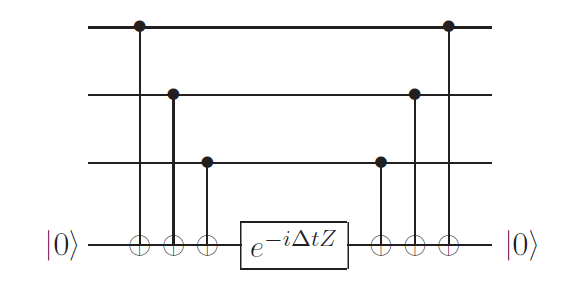
\includegraphics[width = 0.7\textwidth]{images/hamiltonian stuff.png}
    \caption{Circuit for $H = {Z_{1}}\otimes{Z_{2}}\otimes{Z_{3}}$}
\end{figure}
Here's the interesting part, we can execute Hamiltonians which cause a rotation of $\pi$ on the Bloch sphere using this circuit along with basis changing operators. For example if we want $X_{1}$ instead of $Z_{1}$ we can simply put Hadamard on the first bit at the start and at the end and it would work. We can extend it to rotations of arbitrary angles by using a different operator on the ancilla bit. So this way we can execute Hamiltonians of form $H = \sum_{k = 1}^{L}H_{k} + Z^{\otimes{n}}$ or something similar however these usually aren't found in nature.\\
Not all Hamiltonians can be executed efficiently however for example to process of a system achieving equilibrium has no known efficient way of execution also the process by itself is not very well understood. The equilibrium state's density matrix is defined as the Gibb's state and is writen as $\rho_{eq} = e^{-\beta{H}}/Z$ where the partition function $Z = tr(e^{-\beta{H}})$. Note that $\rho_{eq}$ is not provably the actual density matrix of the equilibrium state but rather an educated guess for it.





\chapter{Algorithms for Quantum Computing}
In this chapter I will discuss the algorithms and functionality behind certain algorithms for Quantum Computers.

\section{The Quantum Fourier Transform}
The normal Fourier transform essentially decomposes a signal into it's constituent frequencies. The Quantum Fourier transform in the same idea acts on a $N = 2^n$ dimensional vector $(x_0,x_1,...x_{N-1})$ in $\mathbb{C}^{N}$ and maps it to a vector $(y_0,y_1,...y_{N-1})$ in $\mathbb{C^N}$ according the following formula
$$y_k = \dfrac{1}{\sqrt{N}}\sum_{j = 0}^{N}x_{j}e^{2\pi\iota{jk/N}}$$
Now an important thing to note is that this happens to be a unitary transform which means that we can execute it in a quantum circuit thanks to universality.
Now we can represent each vector in this space with $n$ qubits. Let each state be represented as $\ket{j_1,j_2,...,j_n}$. Let $0.j_1j_2..j_n$ represent the binary representation of the sum of fractions ${j_1}/{2} + .... + {j_n}/{2^n}$. We can see that the Fourier transform over this state can be written as
\begin{equation}U_{QFT}\ket{j_1,j_2,...,j_n} = \dfrac{(\ket{0} + e^{2\pi\iota0.j_n}\ket{1})(\ket{0} + e^{2\pi\iota0.j_{n-1}j_{n}}\ket{1}).....(\ket{0} + e^{2\pi\iota0.j_{1}j_{2}...j_{n}}\ket{1})}{2^{n/2}}\end{equation}
Now if we define a rotation matrix $R_k = \begin{bmatrix}1 & 0\\0 & e^{2\pi\iota/2^k}\end{bmatrix}$ we can create an efficient circuit for executing the Quantum Fourier transform like this (see fig 4.1).
\begin{figure}[ht]
    \centering
    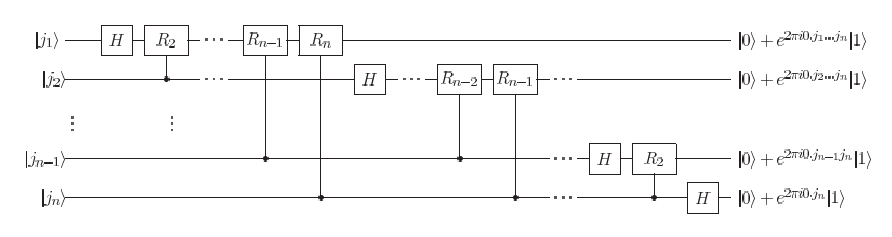
\includegraphics[width = 0.7\textwidth]{images/QFT circuit.png}
    \caption{Circuit for QFT. Note that this does not include the swap gates for reversing order of output qubits and normalization}
\end{figure}
Using this we can do lots of things which classical computers would have taken exponential time for since classical computers would require $\Theta(2^{2n})$ complexity in number of operations and quantum computers only require a $\Theta{(n^2)}$ as seen from fig 4.1 and that is an exponential improvement. Here are some interesting things which can be done using the Fourier transform.

\subsection{Phase estimation}
Suppose we have unitary operator $U$ with an eigen vector $\ket{u}$ with an eigenvalue $e^{2\pi\phi}$ where $\phi$ is unknown and we wish to estimate its value. We us two registers, one which has $t$ qubits and the other which is initialized in state $\ket{u}$. Now lets say that the binary representation of $\phi$ is $0.\phi_1\phi_2...\phi_t$ accurate to $t$ places after the radix point.\\
We will now execute the following circuit described in fig. 4.2.
\begin{figure}[ht]
    \centering
    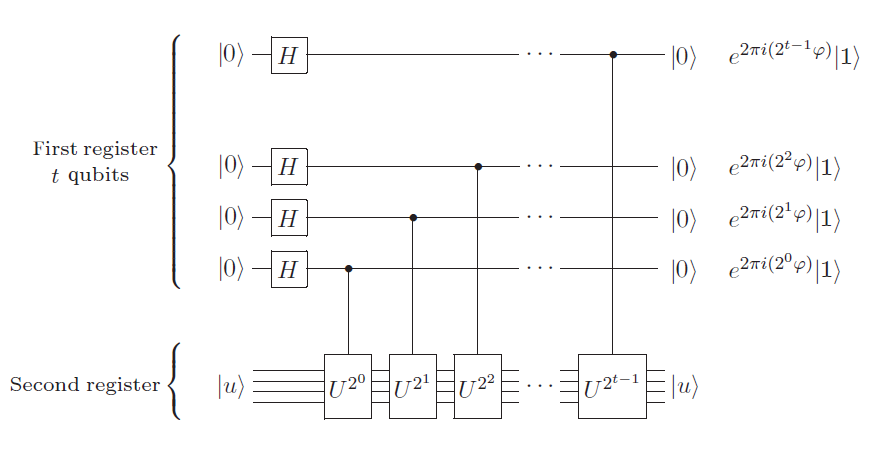
\includegraphics[width = 0.7\textwidth]{images/phase estimation.png}
    \caption{Circuit for phase estimation. Note that we perform inverse Fourier transform on the first register and then a measurement on the first register}
\end{figure}
The state of the first register will now be
$$\dfrac{(\ket{0} + e^{2\pi\iota0.\phi_t}\ket{1})(\ket{0} + e^{2\pi\iota0.\phi_{n-1}\phi_{n}}\ket{1}).....(\ket{0} + e^{2\pi\iota0.\phi_{1}\phi_{2}...\phi_{n}}\ket{1})}{2^{n/2}}$$
Clearly doing an inverse Fourier transform over this will give us the state $\ket{\phi_1\phi_2...\phi_t}$ hence on measurement we will be able to estimate this phase. This will soon prove to be very useful.

\subsection{Order finding and factoring}
Using the phase estimation algorithm we can also use it for order finding and factoring and also order finding and factoring happen to be equivalent problems. For two integers $x$ and $N$ which are co prime we define the order of $x$ modulo $N$ as the least positive integer $r$ such that $x^{r} = 1$(mod $N$). The order finding problem essentially aims to find this $r$ and it is considered to be a hard problem for classical computers since there is no known efficient algorithm for it. Note that $r$ would never exceed $N$ which is trivial to prove.\\
We will now define a unitary which acts like this (note $x$ is coprime to $N$)
$$U\ket{y} = \ket{xy(\text{mod}N)}$$
We can see that the eigen states of $U$ would be written like this
$$\ket{u_s} = \dfrac{1}{\sqrt{r}}\sum_{k = 0}^{r-1}\text{exp}\left[\dfrac{-2\pi\iota{sk}}{r}\right]\ket{x^{k}\text{mod }N}$$
We can see that the eigen values are exp$\left[\dfrac{2\pi\iota{s}}{r}\right]$ for $s$ being an integer from $0$ to $r-1$. We will be executing controlled $U^{2^j}$ so we would need to know an efficient way to execute that but apart from that we would need the states $\ket{u_s}$ but we would need to know $r$ for that but we obviously don't know that however there is a useful property of these states $$\dfrac{1}{\sqrt{r}}\sum_{s = 0}^{r-1}\ket{u_s} = \ket{1}$$
And using this we can see that the following holds for a $t$ qubit register in the state $\ket{z}$ 
$$\ket{z}U^{z_{1}2^{t-1}}U^{z_{2}2^{t-2}}.....U^{z_{t}2^{0}}\ket{1} = \ket{z}\ket{x^z\text{mod }N}$$
On a side note we can also construct a unitary which does addition over modulo $N$ and initialize our state to zero and get a similar construct.
\begin{figure}[ht]
    \centering
    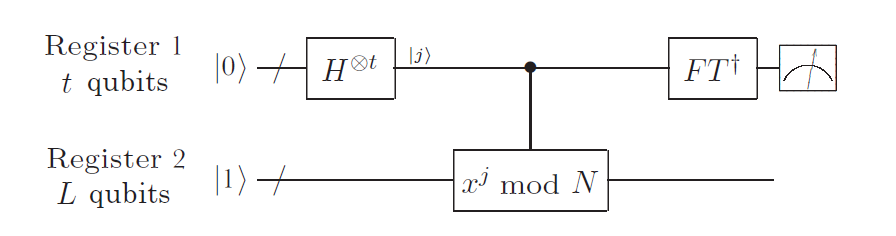
\includegraphics[width = 0.6\textwidth]{images/order finding.png}
    \caption{Circuit for order finding}
\end{figure}
Now to actually obtain the order from this requires use of the continued fractions algorithm. We will only obtain the phase estimate after performing inverse Fourier transform which would be $\phi \approx s/r$. The aim is to find a $s^{'}$ and $r^{'}$ such that $s^{'}/r^{'} = s/r$ and we can verify whether $r^{'}$ is the order by simply calculating $x^r{'}$mod $N$. If $s$ and $r$ are co-prime then we will get $r^{'} = r$ so that is not an issue and also for most possible pairs of $s$ and $r$ however in the case that they aren't co-prime, the best approach is to run the algorithm twice so we will have two fractions $s_{1}^{'}/r_{1}^{'}$ and $s_{2}^{'}/r_{2}^{'}$, if we have $s_{1}^{'} \neq s_{2}^{'}$ we can get $r$ by taking the LCM of $r_{1}^{'},r_{2}^{'}$ and the probability of this being successful is fairly high and can be proved to be greater than 1/4.\\
The order finding algorithm proceeds in the following manner:\\
\textbf{Input: }Black box for executing $U_{x,N}$ which performs the following operation $U_{x,N}\ket{j}\ket{k} = \ket{j}\ket{x^{j}k\text{mod }N}$ for $x$ co-prime to $L$ bit integer $N$. Also $t$ qubits initialized to $\ket{0}$ where $t = 2L + 1 + \ceil{log(2 + \frac{1}{2\epsilon})}$ and an $L$ qubit register set to the state $\ket{1}$.\\
\textbf{Output: } The smallest positive integer $r$ such that $x^r$mod $N$ = 1.\\
\textbf{Procedure:}
\begin{enumerate}
\item Initialize state to $\ket{0}\ket{1}$
\item Create the superposition state $\dfrac{1}{\sqrt{2^t}}\sum_{j=0}^{2^t-1}\ket{j}\ket{1}$ using Hadamard.
\item Apply the black box and the state becomes $\dfrac{1}{\sqrt{2^t}}\sum_{j=0}^{2^t-1}\ket{j}\ket{x^{j}\text{mod }N} \approx \dfrac{1}{\sqrt{r2^t}}\sum_{s=0}^{r-1}\sum_{j=0}^{2^t-1}e^{2\pi\iota{sj}/r}\ket{j}\ket{u_s}$
\item Applying inverse Fourier transform we get the state $\dfrac{1}{\sqrt{r}}\sum_{s=0}^{r-1}\ket{\widetilde{s/r}}\ket{u_s}$
\item Measure the first register to obtain $\widetilde{s/r}$
\item Apply continued fractions algorithm to obtain $r$
\end{enumerate}
Now to prove that the problem of factoring actually reduces to order finding, we use two lemmas. If we have $x^2 = 1$(mod $N$) but $x \neq \pm 1$(mod $N$) then at least one of gcd$(x-1,N)$ and gcd$(x+1,N)$ is a non trivial factor of $N$ and this can be computed in $O(L^3)$ operations.
\\
The second lemma is that suppose we have the prime factorization of an odd composite number $N = p_{1}^{\alpha_1}....p_{m}^{\alpha_m}$. Let $x$ be randomly chosen with requirement $1 \leq x \leq N-1$ and $x$ is co prime to $N$. Let $r$ be the order of $x$ modulo $N$ then the probability of $r$ being even and $x^{r/2} \neq -1$(mod $N$) $\geq 1 - \dfrac{1}{2^m}$\\
Using these two theorems we can obtain an algorithm which returns a non trivial factor of $N$ with high probability and this happens to be Shor's Factoring algorithm. The steps of this algorithm are as follows (note this doesn't outline what exactly is happening in the circuit for this):\\
\textbf{Inputs: }A composite number $N$\\
\textbf{Output: }A non trivial factor of $N$\\
\textbf{Procedure:}
\begin{enumerate}
    \item If $N$ is even just return 2 else continue.
    \item Determine using a classical algorithm whether $N = a^b$ for integers $a \geq 1$ and $b \geq 2$. The classical algorithm finds the value of $y = $log$N$ and then $x = y/b$ for $b \leq L$ and then finds the closest integers to $2^x$ $u_1$ and $u_2$. If either of $u_1^b$ or $u_2^b$ are equal to $N$ then the $N$ has such a representation for integer $a,b$ according to the previous conditions and return $a$ else continue.
    \item Randomly chose $x$ from 1 to $N-1$ and if gcd$(x,N) > 1$ then return gcd$(x,N)$ else continue.
    \item Do the order finding subroutine to find order $r$ of $x$ modulo $N$. \item If $r$ is even and $x^{r/2} = -1($mod $N)$ then compute gcd$(x^{r/2} - 1,N)$ and gcd$(x^{r/2} + 1,N)$, and test to see if one of these is a non-trivial factor, returning that factor if so. Otherwise, the algorithm fails.
\end{enumerate}
This runs in $O(L^3)$ complexity and has a success probability of $O(1)$.
If we try factoring 91 by this algorithm, we can see that the first two steps would be skipped and then if we choose $x = 4$ then we can see that $r = 6$ and $4^{r/2} = 64$mod $91 \neq -1$mod 91 and gcd$(64 - 1,91)$ happens to give 7 so the algorithm succeeds. Though this may not seem very efficient if extrapolated to very large numbers it performs much better than classical algorithms since order finding has no known efficient algorithm for classical computers. This is the famous factoring algorithm which is soon to break RSA encryption according to most websites but that is mostly to be many years later considering the largest number that has been factorized on an actual quantum computer using this algorithm is 21.

\subsection{Period finding}
Another way of using the quantum Fourier transform is for finding the period of a periodic function which means given a function $f(x+r) = f(x)$ for $0 < r < 2^L$
we have to find the value of $r$. The function will be given as a black box which executes this unitary $U\ket{x}\ket{y} = \ket{x}\ket{y \oplus f(x)}$. Using the following algorithm we can find the period of by just using $U$ once.
\textbf{Inputs: }The black box which performs $U$ along with a state to store the function evaluation initialized to $\ket{0}$ and a $t = O(L + \log(1/\epsilon))$ qubit register initialized to $\ket{0}$.\\
\textbf{Output: }The least integer $r > 0$ such that $f(x+r) = f(x)$.\\
\textbf{Procedure:}
\begin{enumerate}
    \item Initialize the state to $\ket{0}\ket{0}$.
    \item Create the superposition state $\dfrac{1}{\sqrt{2^t}}\sum_{x=0}^{2^t-1}\ket{x}\ket{0}$.
    \item Apply the unitary to get this state $\dfrac{1}{\sqrt{2^t}}\sum_{x=0}^{2^t-1}\ket{x}\ket{f(x)} \approx \dfrac{1}{\sqrt{r2^t}}\sum_{l=0}^{r-1}\sum_{x=0}^{2^t-1}e^{2\pi\iota{lx}/r}\ket{j}\ket{\hat{f}(l)}$.
    \item Apply inverse Fourier transform to get $\dfrac{1}{\sqrt{r}}\sum_{l=0}^{r-1}\ket{\widetilde{l/r}}\ket{\hat{f}(l)}$
    \item Measure the register to get $\widetilde{l/r}$.
    \item Apply the continued fractions algorithm to get the value of $r$.
\end{enumerate}
As one can see this bears a lot of similarities to the normal order finding algorithm and interestingly the order finding algorithm is actually just an example of the period finding algorithm since it finds the period of the function $f(x) = a^x\mod N$. Matter of fact $\ket{\hat{f}(l)} = \dfrac{1}{\sqrt{r}}\sum_{l=0}^{r-1}e^{-2\pi\iota{lx}/r}$ which is the Fourier transform of $f(x)$ and we can actually see that it also happens to be the eigen state of $U$ with an eigen value of $l/r$ so we are just doing a phase estimation of that.\\
Now if we define another state $\ket{\tilde{f}(l)} = \dfrac{1}{\sqrt{N}}\sum_{x=0}^{N-1}e^{-2\pi\iota{lx}/N}\ket{f(x)}$ and for the function $f(x+r) = f(x)$ we define a unitary $U_{y}\ket{f(x)} = \ket{f(x+y)}$. We can see that $\ket{\tilde{f}(l)}$ happens to be eigen states of $U_y$ due to the shift invariance property of the Fourier transform and the eigen value would be $e^{2\pi\iota{ly}/N}$. Now if we are given a $\ket{f(x_0)}$ along with the black box for executing $U_y$ we can use it for period finding with some modifications.

\subsection{Discrete logarithms}
The discrete logarithm problem is that if given $a$ and $b = a^s$, we have to determine $s$. So first lets start with a periodic function slightly more complex than the one in the previous subsection. Say we have the function $f(x_1,x_2) = a^{sx_1 + x_2}\mod N$ and let say $r$ is the smallest positive integer $a^r\mod N = 1$. This function's period is a tuple $(l,-ls)$. Say we have a unitary $U\ket{x_1}\ket{x_2}\ket{y} = \ket{x_1}\ket{x_2}\ket{y \oplus f(x_1,x_2)}$ we can actually find its period in a similar manner to the period finding algorithm described in the previous subsection.\\
So we just start with the state $\ket{0}\ket{0}\ket{0}$ over three registers where the first two have $t = O(\ceil{\log r} + \log(1/\epsilon))$ qubits and the third one stores the function and then create the superposition states for the first two register. We then apply the unitary on the state and that can be decomposed in a similar way as shown in step 3 of the period finding algorithms procedure to $$\dfrac{1}{2^t}\sum_{x_1=0}^{2^t-1}\sum_{x_2=0}^{2^t-1}\ket{x_1}\ket{x_2}\ket{f(x_1,x_2)}$$ 
$$\approx \dfrac{1}{2^t\sqrt{r}}\sum_{l_2=0}^{r-1}\sum_{x_1=0}^{2^t-1}\sum_{x_2=0}^{2^t-1}e^{2\pi\iota(sl_2x_1 + l_2x_2)}\ket{x_1}\ket{x_2}\ket{\hat{f}(sl_2,l_1)}$$
\begin{equation}= \dfrac{1}{2^t\sqrt{r}}\sum_{l_2=0}^{r-1}\left[\sum_{x_1=0}^{2^t-1}e^{2\pi\iota(sl_2x_1)}\right]\left[\sum_{x_2=0}^{2^t-1}e^{2\pi\iota(l_2x_2)}\right]\ket{x_1}\ket{x_2}\ket{\hat{f}(sl_2,l_1)}\end{equation}
We can see that applying the inverse Fourier transform and measuring the first two registers will give us $sl_2/r$ and $l_2/r$ from which we can deduce $s$ by using continued fractions algorithm.\\
Note that $\ket{\hat{f}(l_1,l_2)} = \dfrac{1}{\sqrt{r}}\sum_{j=0}^{r-1}e^{-2\pi\iota{l_2j}/r}\ket{f(0,j)}$ which is the Fourier transform of $f(x_1,x_2)$. Note that $l_1,l_2$ must satisfy $\sum_{k=0}^{r-1}e^{2\pi\iota{k(l_1/s - l_2)}/r} = r$ else the amplitude of $f(l_1,l_2)$ would go to zero.\\
Obtaining the value of $s$ from $sl_2/r$ and $l_2/r$ can be done in the following manner. First if we consider the case where $s$ and $r/\gcd(l_2,r)$ are co prime we can simply see that the two fractions we will get by continued fractions algorithm say $s^{'}l_2^{'}/r_1^{'}$ and $l_2^{'}/r_2^{'}$ we can see that $s$ can be obtained since the numerator of first fraction will just be an integer multiple of the second and also their denominators will be the same. The problem arises when $s$ is not co prime with $r/\gcd(l_2,r)$ in which situation we will see that $r_{1}^{'}$ will be a factor of $r_{2}^{'}$ so we can run the algorithm twice since probability that both the times the probability of obtaining the same values becomes very small so we can then take the lcm of the denominators of the different fractions and we have a good probability of obtaining $r$ from that is high since it would just require their numerators to be co prime and then from there we can obtain $s$ by multiplying know fractions by the value of $r$ and then seeing what integer multiple one is of the other.


\subsection{Hidden subgroup problem}
The hidden subgroup problem describes a set of problems of this type: let $f$ be a function from a finitely generated group $G$ to a finite set $X$ such that $f$ is constant on the cosets of a subgroup $K$, and distinct on each coset. Given a quantum black box for performing the unitary transform $U\ket{g}\ket{h} = \ket{g}\ket{h\oplus(g)},$ for $g \in G, h \in X$, and $\oplus$ is an appropriately chosen binary operation on $X$, find a generating set for $K$.\\
Order finding, period finding, discrete logarithms are all instances of the hidden subgroup problem. For the period finding algorithm $G$ is the set of positive integers, and $K = \{r,2r,3r,...\}$ for $r \in G$ with the function $f(x+r) = f(x)$ and $X$ is any finite set. Also one can notice the similarities between all these algorithms so far and they can be generalized for some finite abelian group $G$ (in fact they can also be done for finitely generated abelian groups).\\
The first step is applying a Fourier transform (a generalization of the Hadamard operation) to create a superposition state and over this we apply the black box for $f(x)$ to get the state $\dfrac{1}{\sqrt{|G|}}\sum_{g\in{G}}\ket{g}\ket{f(g)}$. We now express $f(g)$ in it's Fourier basis of $\ket{\hat{f}(l)}$ so the state can be rewritten as 
$$\dfrac{1}{|G|}\sum_{g\in{G}}\sum_{l=0}^{|G|-1}e^{2\pi\iota{lg}/|G|}\ket{g}\ket{\hat{f}(l)}$$
Now this looks very familiar doesn't it? For the $\ket{\hat{f}(l)}$ it will have zero amplitude if $l$ doesn't satisfy $\sum_{h\in{K}}e^{2\pi\iota{lh}/|G|} = |K|$ so now if we can find the $l$ values we can find a generating set for the hidden subgroup $K$ however this is not exactly an easy task since when doing our regular period finding or such tasks we arrange the fraction $l/|G|$ to be such that $l$ and $|G|$ do not have common factors but for some arbitrary $G$ this may not at all be necessary.\\
There is a way however, since abelian groups are isomorphic to a product of cyclic groups of prime power order, that is $G = \mathbb{Z}_{p_1} \times \mathbb{Z}_{p_2} ....\times \mathbb{Z}_{p_m}$ where $\mathbb{Z}_{p_i}$ is a group over integers $\{0,1,...{p_i-1}\}$ with addition modulo over $p_i$ so we can rewrite our phase as
$$e^{2\pi\iota{lg}/|G|} = \prod_{i=1}^{M}e^{2\pi\iota{{l_i}^{'}g_i}/{p_i}}$$
And we can easily find $l_{i}^{'}$ from phase estimation and then solve the hidden subgroup problem. However finding the prime power order groups is a hard problem that is at least as hard as factoring but since we are working with a quantum computer, it can also be used for finding these prime power order groups in efficient time. It is possible to do so since each abelian group has a unique representation of this form and for an abelian group which is the set of integers this really would just boil down to factoring.

\subsection{Deutsch-Josza Algorithm and Simon's Algorithm}
The Deutsch-Josza Algorithm is a fairly famous example of a hidden subgroup problem solving algorithm. The problem it solves goes like this, we are given a function $f(x)$ which takes in a $n$ bit string and outputs either 0 or 1. Now we are given the following as a fact that this function is either a constant function or is a balanced function i.e. it gives the outputs of 0 and 1 an equal number of times. Our goal is to find out whether it is balanced or constant.\\
On a classical computer this would take $2^{n-1}+1$ iterations to conclude however a quantum computer can do much better, it would take only one call of the oracle.
Let the oracle be $U\ket{x}\ket{y} = \ket{x}\ket{y \otimes f(x)}$. We will have two registers one of $n$ qubits and the other of only one qubit. The first register is initialized at $\ket{0}$ and the other is at $\ket{1}$. 
We now apply Hadamard to to both registers so we get this state $\dfrac{1}{\sqrt{2^{n+1}}}\sum_{x=0}^{2^n-1}\ket{x}(\ket{0}-\ket{1})$. We now apply the oracle on this state to get $\dfrac{1}{\sqrt{2^{n+1}}}\sum_{x=0}^{2^n-1}\ket{x}(\ket{f(x)}-\ket{1 \oplus f(x)}) = \dfrac{1}{\sqrt{2^{n+1}}}\sum_{x=0}^{2^n-1}(-1)^{f(x)}\ket{x}(\ket{0}-\ket{1})$\\
We can now just ignore the second register and apply Hadamard on the first register again and we will get $$\frac{1}{2^n}\sum_{y=0}^{2^n-1}\left[\sum_{x=0}^{2^n-1}(-1)^{f(x)}(-1)^{x \cdot y} \right]\vert y\rangle$$
We now perform a measurement on this register but now here's the thing, the probability of measuring the state $\ket{0}$ is 1 if $f(x)$ is constant but 0 if $f(x)$ is balanced so depending on whether we get the state $\ket{0}$ on measurement or not, we will find out the function.\\\\
Simon's algorithm is another such algorithm which solves the problem where we are given a blackbox for a function which is either a one-one function or is a two-one function which does mapping according to some hidden bit string $s$ such that if $f(x_1) = f(x_2)$ then $x_1 \oplus x_2 = s$. Let the domain of this function be over bit strings of $n$ bits then we would have to do $2^{n-1} + 1$ oracle calls on a classical computer but with a quantum computer we can do far better.\\
Now we have our usual unitary $U\ket{x}\ket{y} = \ket{x}\ket{f(x) \oplus y}$ where $\ket{x}$ and $\ket{y}$ are of $n$ qubit registers. The first step is to initialize the whole state to $\ket{0}\ket{0}$ and then apply Hadamard on the first register and then apply the black box for the unitary to get $\dfrac{1}{\sqrt{2^n}}\sum_{x=0}^{2^n-1}\ket{x}\ket{f(x)}$. Now we measure the second register and in the case we have the two one function then we have the state $\dfrac{1}{\sqrt{2}}(\ket{x} + \ket{y})$ when we measure to get $\ket{f(x)}$ for the second register and $y = x \oplus s$. Now we will apply Hadamard again on the first register to get   $\dfrac{1}{\sqrt{2^{n+1}}} \sum_{z \in \{0,1\}^{n} } \left[  (-1)^{x \cdot z} + (-1)^{y \cdot z} \right]  \lvert z \rangle$. On measuring this state, the possible values of $z$ satisfy $x \cdot z = y \cdot z \mod 2$ which reduces to $s \cdot z = 0$ and if we have n distinct values for $z$ obtained we can find out $s$ by Gauss elimination so this can be run at about $n$ oracle calls which is a potential exponential speed up.



\section{Search algorithms}
Now in a classical computer the complexity of searching a list is $O(N)$ quite obviously but there is an algorithm which can do it on a Quantum computer in $O(\sqrt{N})$. Now this may not look as impressive as the exponential speedups which we obtained for Fourier transform and all but it is still quite useful and important.
\subsection{Grover's Search Algorithm}
Now say we have an indexed list of $N = 2^{n}$ elements and we have a function $f(x)$ over this list where $f(x) = 0$ if the element is not the solution and $f(x) = 1$ if it is solution. We are having some $\leq M \leq N$ solutions. We have an oracle which executes the following $O\ket{x}\ket{y} = \ket{x}\ket{y \oplus f(x)}$. So if we have the state $\ket{x}\ket{-}$ where $\ket{-} = \dfrac{1}{\sqrt{2}}(\ket{0} - \ket{1})$ then applying $O$ gives us $(-1)^{f(x)}\ket{x}\ket{-}$ so we can just ignore the second qubit and see that it makes $\ket{x}$ go to $(-1)^{f(x)}\ket{x}$.\\
An important point to address here is the construction of the oracle itself. If we can construct the oracle then that means we know the solutions, so then what are we searching for? Now knowing the solution and searching for it are two very different things as the goal here is to find the known solutions from the indexed list of elements. The key point is, an oracle which recognizes the solutions to a problem can be constructed without actual knowledge of the solutions and this will be our main principle in utilising this search algorithm.\\
For describing our circuit we will first define a Grover operator $G$ which does the following (shown in fig 4.4)
\begin{figure}[ht]
    \centering
    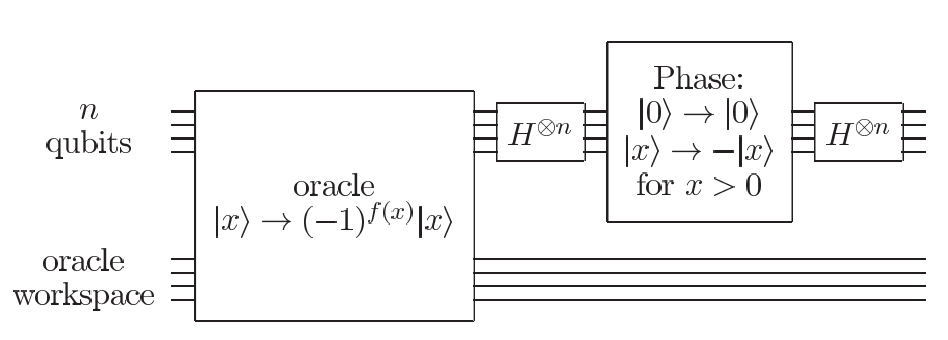
\includegraphics[width = 0.7\textwidth]{images/grover iteration.png}
    \caption{Grover iteration}
\end{figure}
The phase happens to have the unitary $2\ket{0}\bra{0} - 1$ and on applying the Hadamard on both sides $H^{\otimes N}(2\ket{0}\bra{0}-1)H^{\otimes N} = 2\ket{\psi}\bra{\psi}-1$ where $\ket{\psi}$ is the superposition state. From this we can see
$$G = (2\ket{\psi}\bra{\psi} - 1)O$$
An interesting thing to note is that the unitary $2\ket{\psi}\bra{\psi} - 1$ will produce an inversion about mean in the sense that only the component of the state that is parallel to the superposition has it's sign unchanged. This brings us to the geometric visualization of the Grover's algorithm.\\
So we will now define $\ket{\alpha} = \dfrac{1}{\sqrt{N-M}}\sum_{x|f(x)=0}\ket{x}$ and $\ket{\beta} = \dfrac{1}{\sqrt{M}}\sum_{x|f(x)=1}\ket{x}$. So we write
\begin{equation}\ket{\psi} = \sqrt{\dfrac{N-M}{N}}\ket{\alpha} + \sqrt{\dfrac{M}{N}}\ket{\beta}\end{equation}
Now let $\ket{\psi} = \cos\left(\dfrac{\theta}{2}\right)\ket{\alpha} + \sin\left(\dfrac{\theta}{2}\right)\ket{\beta}$, we can observe the following to hold
\begin{equation}G^{k}\ket{\psi} = \cos\left(\dfrac{2k+1}{2}\theta\right)\ket{\alpha} + \sin\left(\dfrac{2k+1}{2}\theta\right)\ket{\beta}\end{equation}
This shows that $G$ just happens to be a rotation in $\ket{\alpha},\ket{\beta}$ space. The core idea of the search algorithm is to rotate $\ket{\psi}$ till it approaches $\ket{\beta}$ so essentially it would make the state into being composed of the solutions. The fig 4.5 describes the rotation idea.
\begin{figure}[ht]
    \centering
    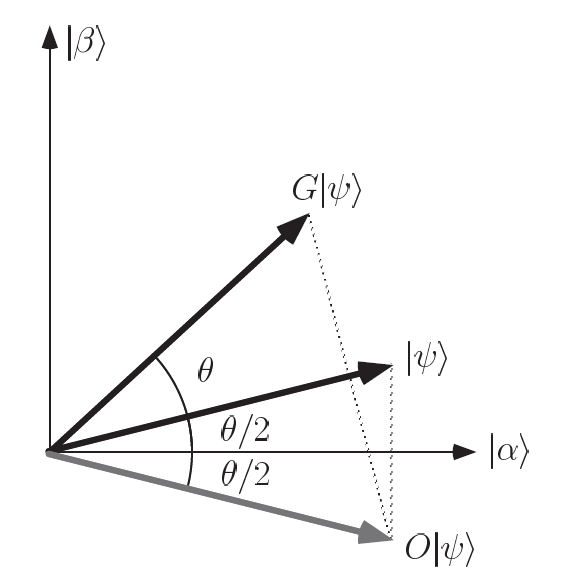
\includegraphics[width = 0.4\textwidth]{images/rotation grover.png}
    \caption{Grover rotation}
\end{figure}
Now the very important question is that how many times must we apply the operation to obtain a close estimate of $\ket{\beta}$. We can see that doing these many iterations will give us the needed state. 
$$R = \text{Round}\left(\dfrac{\arccos{\sqrt{M/N}}}{\theta}\right)$$
Here Round is a function which rounds up to the nearest integer and rounds halves down. An important thing to see here is that the error will be very small if we have $M << N$. Now at the moment if we assume that $M \leq N/2$ then since $\theta/2 \geq \sin(\theta/2)$ we obtain the upper bound 
\begin{equation}R \leq \left\lceil{\dfrac{\pi}{4}\sqrt{\dfrac{N}{M}}}\right\rceil\end{equation}
Now this makes things a lot more convenient as we just need the number of solutions and not the actual values of them and this is where we obtain the term for complexity of circuit as $O(\sqrt{N/M})$.\\
The algorithm procedes like this, we start with the state $\ket{0}^{\otimes{n}}\ket{0}$. We now apply Hadamard on the first register of $n$ qubits and $HX$ on the second register of 1 qubit. We now have the state $\dfrac{1}{\sqrt{2^{n+1}}}\sum_{x=0}^{2^{n}-1}\ket{x}(\ket{0} - \ket{1})$. Now we apply the Grover iteration for $R \approx \left\lceil{\dfrac{\pi}{4}\sqrt{\dfrac{N}{M}}}\right\rceil$ and we will obtain an approximate state to $\ket{\beta}$ in the first register and we would have to approximately measure $M$ times to know all the solutions. Now if we have $M \geq N/2$ then we simply add another qubit which would essentially double our $N$ so it just goes back to $M \leq N/2$ case. Funnily according to formula of $R$ we mentioned previously, when $M$ increases from $N/2$ to $N$ it would increase the number of iterations. However introducing another qubit would require us to change the oracle. The new oracle can actually be shown to be this circuit in fig. 4.6 however it requires two ancillary qubits. 
\begin{figure}[ht]
    \centering
    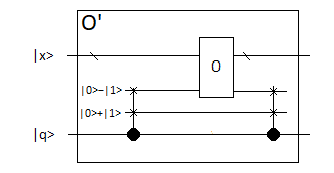
\includegraphics[width = 0.6\textwidth]{images/oracle stuff.png}
    \caption{New oracle with the extra qubit}
\end{figure}
Given that this algorithm speeds up the search process it has a ton of applications given the fact that a lot of algorithms utilise a search. While the speedup is only polynomial and not exponential it is still very useful especially for speeding up an NP-complete problem. One such problem is the Hamiltonian cycle problem.\\
This is a problem which examines a graph and tells whether it has a Hamiltonian cycle or not where a Hamiltonian cycle is a cycle through the graph where every vertex is visited once. It is widely believed to be NP-complete but it has not been proven yet. The classical algorithm goes like this:\\
(1) Find every possible ordering of the vertices $(v_1,....v_n)$ of the graph while allowing repetitions as they ease the analysis.\\
(2) If a certain permutation works then there is a Hamiltonian cycle else continue searching.\\ 
Since there are $n^n = 2^(n\log{n})$ orderings possible we just need a search among these elements. Let $m = \ceil{\log{n}}$ then we have to do a search using $nm$ qubits and have some oracle which does $O\ket{v_1,....v_n} = \ket{v_1,....v_n}$ if it isn't a Hamiltonian cycle and $O\ket{v_1,....v_n} = -\ket{v_1,....v_n}$ if it is and as we know this method will require complexity of $O(2^{mn/2})$ which is a speedup over the classical approach.


\subsection{Hamiltonian for search algorithm}
Now this algorithm looks real good and all but how did we reach here? For explaining the approach we will start with some state $\ket{\psi}$ and find a Hamiltonian which will evolve this state to $\ket{x}$ where this state is the solution (for now lets just assume one solution) in some time $\Delta{t}$. Once we find this Hamiltonian we simply construct a circuit for simulating it.\\
Now if we begin making guesses for the Hamiltonians we can see that the terms would be constructed with $\ket{\psi}$ and $\ket{x}$. Now we write two Hamiltonians
\begin{equation}H = \ket{x}\bra{x} + \ket{\psi}\bra{\psi}\end{equation}
\begin{equation}H = \ket{x}\bra{\psi} + \ket{\psi}\bra{x}\end{equation}
Now the interesting thing is that both of these can be used to describe the search Hamiltonian but for now we will focus on the one in eq. 4.6. Now we just have to run this simulation till time $t$ for which $\exp(-\iota{Ht})\ket{\psi} = \ket{x}$. Now if we take $\ket{x}$ and $\ket{y}$ to be the orthonormal basis of this space then we can write $\ket{\psi} = \alpha\ket{x} + \beta\ket{y}$ where $\alpha^2 + \beta^2 = 1$. When we write $H$ in this basis we get $H = I + \alpha(\beta{X} + \alpha{Z})$. We can see that 
$$\exp(-\iota{Ht})\ket{\psi} = \exp(\iota{t})[\cos(\alpha{t})\ket{\psi} - \iota{\sin(\alpha{t})}\ket{x}]$$
Now we can simply ignore the phase factor and note that for $t = \pi/2\alpha$ we will get the result $\ket{x}$ on measurement with unity probability. Now this unfortunately depends on the quantity $\alpha$ which is dependent on $\ket{\psi}$ and $\ket{x}$ but if we choose $\ket{\psi}$ to be the uniform superposition state then we know that $\alpha$ will be the same for all choices of $\ket{x}$ and Voila! This is pretty much how the search algorithm works!\\
Alright so that's all good but what about the circuit? Well we just need to follow the method described in section 3.3 and we can see the following circuits can be used
\begin{figure}[ht]
\centering
\begin{minipage}{.5\textwidth}
\centering
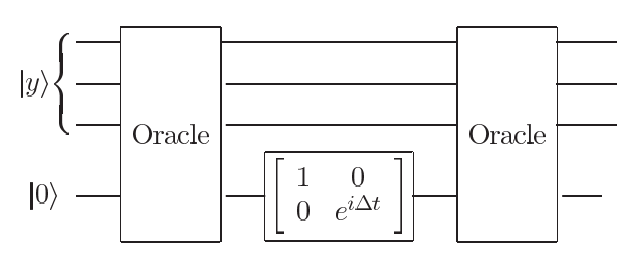
\includegraphics[width=\linewidth]{images/grover hamiltonian x.png}
\captionof{figure}{Circuit for executing exp($-\iota\ket{x}\bra{x}\Delta{t}$)}
\label{fig:x stuff}
\end{minipage}%
\begin{minipage}{.5\textwidth}
\centering
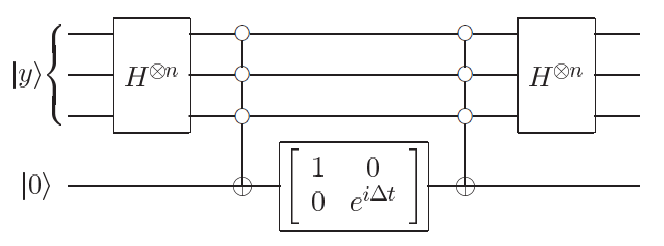
\includegraphics[width=\linewidth]{images/grover hamiltonian psi.png}
\captionof{figure}{Circuit for executing exp($-\iota\ket{\psi}\bra{\psi}\Delta{t}$)}
\label{fig:psi stuff}
\end{minipage}
\end{figure}
The complexity of the circuit will depend on the accuracy we are aiming which will decide how small the time steps we will choose. We can see that if we wish to have an accuracy of $O(\Delta{t^r})$ the cumulative error will come out to be $O(\Delta{t^r}\sqrt{N})$ and since we want the error to be $O(1)$ we choose $\Delta{t} = \Theta(N^{-1/2(r-1)})$ so then we have the number of steps to be $t/\Delta{t}$ and the complexity of the whole circuit will be $O(\sqrt{N} \times N^{1/2(r-1)})$ which gives us $O(N^{r/2(r-1)})$ and we can see that the limit goes to $O(\sqrt{N})$ for $r$ tending to infinity.\\
A thing to note is that here in the analysis of $\Delta{t}$ we have used very general methods and we can use a specific choice to actually do much better. Let us define a $U(\Delta{t}) = \exp(-\iota\ket{\psi}\bra{\psi}\Delta{t})\exp(-\iota\ket{x}\bra{x}\Delta{t})$ on doing a simple calculation we get the following for $U(\Delta{t})$ (note $\ket{x} = \hat{z}$ in this basis)
\begin{equation}
U(\Delta{t}) = \left(\cos^{2}\left(\dfrac{\Delta{t}}{2}\right) - \sin^{2}\left(\dfrac{\Delta{t}}{2}\right)\vec{\psi}\cdot\hat{z}\right)I - 2\iota\sin\left(\dfrac{\Delta{t}}{2}\right)\left(\cos\left(\dfrac{\Delta{t}}{2}\right)\dfrac{\vec{\psi} + \hat{z}}{2} + \sin\left(\dfrac{\Delta{t}}{2}\right)\dfrac{\vec{\psi}\times\hat{z}}{2}\right)
\end{equation}
Here $\vec{\psi} = (2\alpha\beta,0,(\alpha^2-\beta^2))$ which is just the Bloch sphere representation. Now we can see that $U(\Delta{t})$ describes a rotation about some axis in the Bloch sphere. On more observation we can see that it rotates about the axis $\vec{r} = \cos\left(\dfrac{\Delta{t}}{2}\right)\dfrac{\vec{\psi} + \hat{z}}{2} + \sin\left(\dfrac{\Delta{t}}{2}\right)\dfrac{\vec{\psi}\times\hat{z}}{2}$ by an angle $\theta$ such that $\cos\left(\dfrac{\theta}{2}\right) = \cos^{2}\left(\dfrac{\Delta{t}}{2}\right) - \sin^{2}\left(\dfrac{\Delta{t}}{2}\right)\vec{\psi}\cdot\hat{z}$\\
We can also see that $\vec{\psi}\cdot\vec{r} = \hat{z}\cdot\vec{r}$ so a rotation about the axis $\vec{r}$ will make $\vec{\psi}$ go to $\hat{z}$ and the angle for rotation is $\theta$ for which $\cos\left(\dfrac{\theta}{2}\right) = 1 - \dfrac{2}{N}\sin^{2}\left(\dfrac{\Delta{t}}{2}\right)$.\\
Now initially we took $\Delta{t}$ to be small but if we put it as $\pi$ we maximize the rotation angle and that way we get $\theta \approx 4/\sqrt{N}$ and the number of oracle calls would be $O(\sqrt{N})$ and in fact if we put $\Delta{t} = \pi$ we actually get the Grover iteration with $\exp(-\iota\ket{\psi}\bra{\psi}\Delta{t}) = I - 2\ket{\psi}\bra{\psi}$ and $\exp(-\iota\ket{x}\bra{x}\Delta{t}) = I - 2\ket{x}\bra{x}$.\\
In the case of multiple solutions we can use the very same approach by just changing $\ket{x}$ to the superposition of the solutions and we would approach the same Grover iteration idea.

\subsection{Quantum Counting}
An important thing to note about Grover's algorithm is that it requires us to know the number of solutions but what about the case where we do not know this? Here we use phase estimation for this. So we want to estimate the eigen values of the Grover iteration for this.\\
Firstly let's take the appended oracle approach so we can be sure about $M \leq N/2$. From Eq. 4.4 we can see that since $G$ is just a rotation operator, its eigen values are $e^{\iota\theta}$ and $e^{\iota(2\pi-\theta)}$ and $\sin^2(\theta/2) = M/2N$.
\begin{figure}[ht]
    \centering
    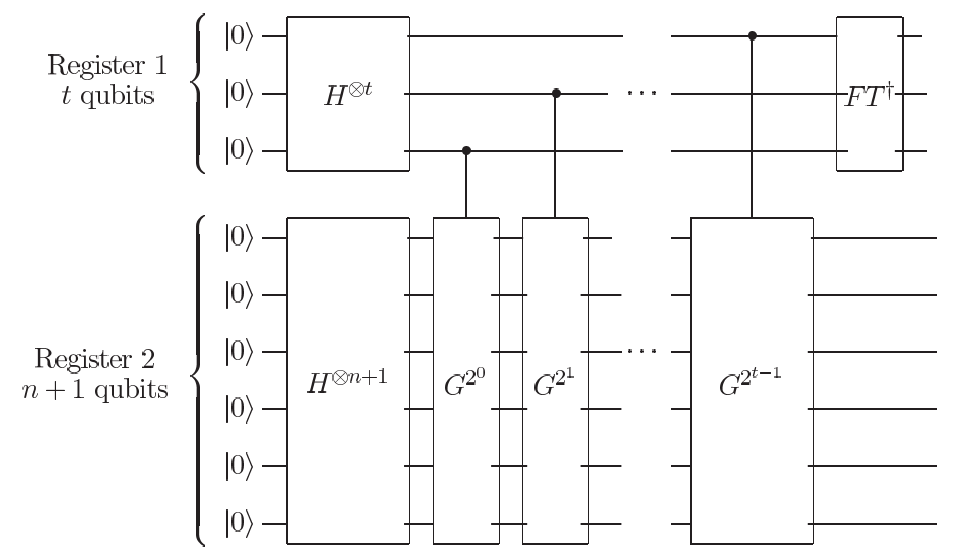
\includegraphics[width = 0.7\textwidth]{images/grover phase estimation.png}
    \caption{Phase estimation for quantum counting}
\end{figure}
Here $t = m + \ceil{\log(2 + 1/2\epsilon)}$ where we want to estimate $\theta$ to an accuracy of $m$ bits so $|\Delta{\theta}| \leq 2^{-m}$ and a probability of $1-\epsilon$. Now we will get some error for $M$ which will be $|\Delta{M}|$
\begin{equation}\dfrac{|\Delta{M}|}{2N} = \left|\sin^2\left(\dfrac{\theta + \Delta{\theta}}{2}\right) - \sin^2\left(\dfrac{\theta}{2}\right)\right|\end{equation}
\begin{equation}\dfrac{|\Delta{M}|}{2N} < \left(2\sin\left(\dfrac{\theta}{2}\right) + \dfrac{\Delta\theta}{2}\right)\dfrac{|\Delta\theta|}{2}\end{equation}
Substituting $\sin^2(\theta/2) = M/2N$ and $|\Delta{\theta}| \leq 2^{-m}$ we have
\begin{equation}\dfrac{|\Delta{M}|}{2N} < \left(\sqrt{2MN} + \dfrac{N}{2^{m+1}}\right)2^{-m}\end{equation}
We can in $\Theta(\sqrt{N})$ oracle calls get our accuracy to be $O(\sqrt{M})$ and this is a clear improvement over the classical approach which would require $O(N)$ oracle calls. Also when we run this along with using the Grover's algorithm if we take $m = \ceil{n/2} + 1$ we get an angular error for $R$ as $\pi/4(1+ |\Delta\theta|/\theta) = \pi/4 \times 3/2 = 3\pi/8$ and combining with success probability of the phase estimation for $\epsilon = 1/6$ we get a success probability of $5/6 \times \cos^2{3\pi/8} \approx 0.12$ which can be improved by a few repetitions of the combined search procedure.

\subsection{Searching an unstructured database}
So far we have conducted searches on structured databases but now we will demonstrate that we can get a speedup even on an unstructured database. We define our problem as follows, we have a database of $N = 2^{n}$ elements labeled as $d_1,d_2,...d_N$ each of which are $l$ bit strings and we wish to find a specific string $s$.\\
When we are running this on a classical computer we consider it to have two components, a CPU where data manipulation is done and it has a small temporary memory and then there is a large memory which stores the database. The CPU can access data from the memory and store it and manipulate it. The method used here is that the elements are given an $n$ bit index for each of them where $n = \ceil{\log{N}}$ and we start with 0 and in each iteration we take one element from the large memory to the CPU and check if it is the required string. If it is then we stop else we continue to the next index and repeat. This is very clearly the most efficient algorithm for a classical computer.\\
For a Quantum computer we can use a similar architecture of a CPU and a memory. This CPU has 4 registers, (1) an $n$ qubit register initialized to $\ket{0}$, (2) an $l$ qubit register initialized to $\ket{s}$ which remains in that for the rest of the computation, (3) Another $l$ qubit register initialized to $\ket{0}$ and (4) a 1 qubit register initialized to $\ket{-}$.\\
The load operation will take the state $\ket{x}\ket{s}\ket{d}\ket{-}$ to $\ket{x}\ket{s}\ket{d \oplus d_x}\ket{-}$ so just we go from $\ket{x}\ket{s}\ket{0}\ket{-}$ to $\ket{x}\ket{s}\ket{d_x}\ket{-}$ and our oracle takes $\ket{x}\ket{s}\ket{d_x}\ket{-}$ to $-\ket{x}\ket{s}\ket{d_x}\ket{-}$ if $d_x = s$ else it does nothing.The addressing scheme will be a quantum addressing scheme also. An important thing to note is that we can load all the data as a superposition and will do the search in $O(\sqrt{N})$ operations but the amount of resources needed for storing the data is pretty much the same as that of a classical computer but these resources are far more cheaper for a classical computer which makes this not all that economically viable also the Grover's algorithm has better uses as speeding up NP complete problems like the Hamiltonian cycle problem.

\subsection{Optimality of the algorithm and Black box limits}
Now we know that the search algorithm requires $O(\sqrt{N})$ queries but it turns out that we cannot actually do any better than that. Suppose we start with some $\ket{\psi}$ and for the sake of simplicity we stick to one solution $\ket{x}$ and our oracles $O_x = I - 2\ket{x}\bra{x}$ and we use the oracle exactly $k$ times and perform $U_1,U_2,...U_k$ between each of these oracles. We now define 
\begin{equation}\ket{\psi_{k}^{x}} = U_{k}O_{x}U_{k-1}O_{x}....U_{1}O_x\ket{\psi}\end{equation}
\begin{equation}\ket{\psi_{k}} = U_{k}U_{k-1}....U_{1}\ket{\psi}\end{equation}
Our goal is to bound the quantity $D_k = \sum_{x}||\ket{\psi_{k}^{x}} - \ket{\psi_{k}}||^2$ which is essentially the deviation after $k$ steps without using the oracles. If $D_k$ is small then the states would be very hard to distinguish in between so this gives us a clue of how much oracles are required to be used.\\
We now prove inductively $D_k \leq 4k^2$
\begin{equation}D_{k+1} = \sum_{x}||O_x(\ket{\psi_{k}^{x}} - \ket{\psi_{k}}) + (O_x - I)\ket{\psi_k}||^2\end{equation}
We can write $(O_x - I)\ket{\psi_k} = -2\ket{x}{\psi_k}\rangle\ket{x}$
\begin{equation}D_{k+1} \leq \sum_{x}(||(\ket{\psi_{k}^{x}} - \ket{\psi_{k}})||^2 + 4||(\ket{\psi_{k}^{x}} - \ket{\psi_{k}})||\text{ }|\bra{x}{\psi_k}\rangle| + 4|\bra{x}{\psi_k}\rangle|^2)\end{equation}
Applying Cauchy Shwarz inequality on the second term on RHS and noting $\sum_{x}|\bra{x}{\psi_k}\rangle|^2 = 1$ gives us
\begin{equation}D_{k+1} \leq D_k + 4\left(\sum_{x}||(\ket{\psi_{k}^{x}} - \ket{\psi_{k}})||^2\right)^{\frac{1}{2}}\left(\sum_{x}|\bra{x}{\psi_k}\rangle|^2\right)^{\frac{1}{2}} + 4\end{equation}
\begin{equation}D_{k+1} \leq D_k + 4\sqrt{D_k} + 4\end{equation}
Clearly if we assume $D_k \leq 4k^2$ then we get from eq. 4.17 that $D_{k+1} \leq 4(k+1)^2$. Now lets assume that $|\bra{x}\psi_{k}^{x}\rangle|^2 \geq 1/2$ so we get our search result at least with 0.5 probability. We now define $E_k = \sum_x||\ket{\psi_{k}^x} - \ket{x}||^2$ and $F_k = \sum_x||\ket{x} - \ket{\psi_k}||^2$. We can see that $E_k \leq (2 - \sqrt{2})N$ since $||\ket{\psi_{k}^x} - \ket{x}||^2 = 2 - 2|\langle{x}|\psi_{k}^{x}\rangle|$ and also $F_k \geq 2N - 2\sqrt{N}$ which we can obtain using the Cauchy Shwarz inequality. We know
\begin{equation}D_k = \sum_{x}||(\ket{\psi_{k}^{x}} - \ket{x}) + (\ket{x} - \ket{\psi_{k}})||^2\end{equation}
\begin{equation}D_k \geq \sum_{x}||\ket{\psi_{k}^{x}} - \ket{x}||^2 + \sum_{x}||\ket{x} - \ket{\psi_{k}}||^2 - 2\sum_{x}||\ket{\psi_{k}^{x}} - \ket{x}||\text{ }||\ket{x} - \ket{\psi_{k}}||\end{equation}
From Cauchy Shwarz inequality we know $\sum_{x}||\ket{\psi_{k}^{x}} - \ket{x}||\text{ }||\ket{x} - \ket{\psi_{k}}|| \leq \sqrt{E_kF_k}$ so we can write eq 4.19 as
\begin{equation}D_k \geq E_k + F_k - 2\sqrt{E_kF_k} = (\sqrt{E_k} - \sqrt{F_k})^2\end{equation}
Now if we use the inequalities of $E_k$ and $F_k$ we get that $D_k \geq cN$ when $N$ is sufficiently large and $c$ is any constant lower than $(\sqrt{2} - \sqrt{2 - \sqrt{2}})^2 \approx 0.42$ and since we established $D_k \leq 4k^2$ we get that $k \geq \sqrt{cN/4}$ so we can see that we get the complexity of $O(\sqrt{N})$ however we cannot get a greater improvement clearly.\\
While this means that we found the best possible quantum search algorithm, it also means that we cannot get a speedup like that of $O(\log N)$ which would be a dream result. Many researchers believe that NP - complete problems involve unstructured searches so a speedy search algorithm can help solve this but this would be pretty bad for Quantum computing since then it would mean that BPQ does not contain NP complete however that is not necessary since factoring which is a little more difficult than NP but not NP complete (a class called NPI) has an efficient implementation here so it might just be a matter of time till we find some quantum approach for NP complete.\\\\
Now if we were to define the decision problem for whether a solution exists or not i.e. given $f(x)$ of the oracle does there exist $x$ such that $f(x) = 1$. $F(X) = X_0 \vee X_1 \vee ... \vee X_{n-1}$ where $X_k = f(k)$. This decision problem can be shown to be equivalent to the search problem for the given oracle itself. Now if we try to generalize this $F(X)$ for operations other than $OR$ to even go over for $AND$, $PARITY$, $MAJORITY$ we obtain some interesting limits for quantum query complexity.\\
Let the deterministic quesry complexity be $D(F)$ and the equivalent for quantum computers we can take to be $Q_E(F)$. The quantity we are concerned with is $Q_2(F)$ which is the query complexity for an accuracy of 2/3. This 2/3 is just arbitrarily chosen since our only concern is to have it larger than 1/2 so we can make it tend to 1 after running it multiple times. Note that $Q_2(F) \leq Q_E(F) \leq D(F) \leq N$. Now since these are boolean functions, we have $X_{k}^{2} = X_{k}$ so using this we can define the minimum degree polynomial of $F(X)$ as $p(X)$
\begin{equation}p(X) = \sum_{Y \in \{0,1\}^N}F(Y)\prod_{k=0}^{N-1}\left[1 - (Y_k - X_k)^2\right]\end{equation}
Quite trivially this will be a unique representation otherwise it wouldn't be the minimum degree polynomial. We will denote the minimum degree of $F(X)$ as deg$(F)$. The degree of $OR$, $AND$, $PARITY$ are actually $N$ and in fact most functions have degree of order $N$ and it has also been proven that
\begin{equation}D(F) \leq 2\text{deg}(F)^4\end{equation}and also 
\begin{equation}D(F) \leq 216\text{deg}(F)^6\end{equation}\\
Now let us take the situation where we have performed $T$ oracle queries in the quantum computer so our state is now $\sum_{k=0}^{2^n-1}c_k\ket{k}$. We will prove that $c_k$ are polynomials of at most degree $T$. Let us start with the state $\ket{\psi_0} = \sum_{ij}\left(a_{i0j}\ket{i}\ket{0} + a_{i1j}\ket{i}\ket{1}\right)\ket{j}$ where the first label is of $n$ qubit register followed by a 1 qubit register and then a $m-n-1$ qubit register. After the oracle query we will obtain $\ket{\psi_1} = \sum_{ij}\left(a_{i0j}\ket{i}\ket{X_i} + a_{i1j}\ket{i}\ket{X_i \oplus1}\right)\ket{j}$ which we can write as
\begin{equation}\ket{\psi_1} = \sum_{ij}\big[\left((1-X_i)a_{i0j} + X_ia_{i1j}\right)\ket{i0} + \left((1-X_i)a_{i1j} + X_ia_{i0j}\right)\ket{i1}\big]\ket{j}\end{equation}
An important point to note is that the in between unitary operations do not change the degree and also here we can see in eq. 4.24 that the coefficients are of degree 1 and on extending this we can see that the coefficients after $T$ queries will be of order less than or equal to $T$. The probability of any of the states would be $|c_k|^2$ which would be of degree less than or equal to $2T$ and so the total probability of obtaining a 1 from the oracle would also be a polynomial of degree at most $2T$ since it is just the sum over the subsets of these probabilities.\\
This probability polynomial would equal $F(X)$ in the case where we are certain of having executed $F(X)$ so we would get deg$(F) \leq 2T$ so we get $Q_E(F) \geq $deg$(F)/2$ and if we have that the probability polynomial approximates $F(X)$ it still would have the same limits on degree so we also get $Q_2(F) \geq $deg$(F)/2$ and from eq. 4.22 and 4.23 we get
$$Q_E(F) \geq \left[\dfrac{D(F)}{32}\right]^{1/4},\text{  } Q_2(F) \geq \left[\dfrac{D(F)}{13824}\right]^{1/6}$$
So as we can see that without modifying the black box itself we cannot achieve anything faster than a polynomial speedup for this kind of problems.

\subsection{Interesting applications of Grover's algorithm}
Apart from also being used for speeding up NP complete problems, we can also develop an algorithm for finding the smallest number from a set of $N$ numbers which are indexed as $T[i]$ for $i \in {0,1..N-1}$
The procedure for it goes something like this when we assume a success probability of 1/2:
\begin{enumerate}
    \item Choose threshold index $0\leq y\leq N-1$ uniformly at random.
    \item Repeat the following and interrupt it when the
    total running time is more than $22.5\sqrt{N} + 1.4\log^{2}N$. Then go to stage 2(c).
    \begin{enumerate}
        \item Initialize the memory as $\sum_{j}\dfrac{1}{N}\ket{j}\ket{y}$. Mark every item j for which $T[j] < T[y]$.
        \item Apply the quantum exponential searching algorithm of [2].
        \item Observe the first register: let $y'$ be the outcome. If $T[y'] < T[y]$, then set threshold index $y$ to $y'$.
    \end{enumerate}
    \item Return $y$.
\end{enumerate}
For the step 2(a) it would in convention take $\log{N}$ steps an the search algorithm we use has complexity of $O(\sqrt{N})$ as we have already established so for a large $N$ the complexity is $O(\sqrt{N})$  also the algorithm would on average require $O(\log(N)\sqrt{N})$ accesses to the database. It must be noted that the algorithm can run infinitely long so we will call that case the infinite algorithm There are some lemmas of this we can see:\\
\textbf{Lemma 1: }\textit{Let p(t,r) be the probability that the index of the element of rank r will ever be chosen when the infinite algorithm searches among t elements. Then p(t,r) = 1/r if $r \leq t$, and p(t,r) = 0 otherwise}\\
For $r > t$ it is trivial. We can prove this using induction for $r \leq t$. Lets assume $p(k,r) = 1/r$ for $k \in [r,t]$ if we mark $t+1$ elements then we have
$$p(t+1,r) = \dfrac{1}{t+1} + \sum_{k=r+1}^{t+1}\dfrac{1}{t+1}p(k-1,r) = \dfrac{1}{r}$$
\textbf{Lemma 2: }\textit{The expected total time used by the infinite algorithm before y holds the index of the minimum is at most $m_0 = \dfrac{45}{4}\sqrt{N} + \dfrac{7}{10}\log^2N$}\\
The expected number of iterations used by the exponential searching algorithm is at most $\frac{9}{2}\sqrt{N/t}$ for finding the index of marked item. So the expected number of minimum steps would be
$$\sum_{r=2}^{N}p(N,r)\dfrac{9}{2}\sqrt{\dfrac{N}{r-1}} = \dfrac{9}{2}\sqrt{N}\sum_{r=1}^{N-1}\dfrac{1}{r+1}\dfrac{1}{\sqrt{r}}$$
$$\sum_{r=2}^{N}p(N,r)\dfrac{9}{2}\sqrt{\dfrac{N}{r-1}} \leq \dfrac{9}{2}\sqrt{N}\left(\dfrac{1}{2} + \sum_{r=2}^{N-1}r^{-3/2}\right) \leq \dfrac{9}{2}\sqrt{N}\left(\dfrac{1}{2} + \int_{r=2}^{N-1}r^{-3/2}\right) \leq \dfrac{45}{4}\sqrt{N}$$
The expected number of steps from stage 2(a) before $T[y]$ hold the minimum is at most
$$\sum_{r=2}^{N}p(N,r)\log{N} = (H_N - 1)\log{N} \leq \ln{N}\log{N} \leq 0.7\log^2N$$
Here $H_N$ is the $N$th harmonic number. After at most $2m_0$ iterations $T[y]$ will hold the value with a probability of 1/2 so here we can see why this only requires $O(\sqrt{N})$ complexity. Refer no. 12 in references for more about this algorithm.



\chapter*{References and other links}
\addcontentsline{toc}{chapter}{References and other links}
\begin{enumerate}
    \item \textit{Quantum Computation and Quantum Information} by Isaac Chuang and Michael Nielsen.
    \item \textit{Qiskit Textbook} of IBM available \href{https://qiskit.org/textbook/preface.html}{here}.
    \item \textit{Quantum Information Science 1, Part 1} edX course available \href{https://courses.edx.org/courses/course-v1:MITx+8.370.1x+1T2018/course/}{here}.
    \item \textit{Notes on Bloch Sphere} available \href{http://web.cecs.pdx.edu/~mperkows/june2007/bloch-sphere.pdf}{here}.
    \item \textit{Notes on Schmidt Decomposition} available  \href{http://users.ox.ac.uk/~kch/demos/quantc7/fqt07w7.pdf}{here}.
    \item \textit{The original EPR paper} available \href{https://journals.aps.org/pr/pdf/10.1103/PhysRev.47.777}{here} and the \href{https://en.wikipedia.org/wiki/EPR_paradox}{wikipedia article}.
    \item \textit{On the Einstein Podolsky Rosen Paradox} by J.S. Bell available \href{https://cds.cern.ch/record/111654/files/vol1p195-200_001.pdf}{here}.
    \item \textit{Tsirelon's Bound} wikipedia article available \href{https://en.wikipedia.org/wiki/Tsirelson\%27s_bound}{here}.
    \item \textit{Using Quantum Gates instead of ancilla bits} acrticle available  \href{https://algassert.com/circuits/2015/06/22/Using-Quantum-Gates-instead-of-Ancilla-Bits.html}{here}.
    \item \textit{Elementary gates for quantum computation} by Adriano Barenco, Charles H. Bennett, Richard Cleve, David P. DiVincenzo, Norman Margolus, Peter Shor, Tycho Sleator, John Smolin,and Harald Weinfurter available \href{https://arxiv.org/pdf/quant-ph/9503016.pdf}{here}.
    \item \textit{The Hidden Subgroup Problem and Eigenvalue Estimation on a Quantum Computer} by Michele Mosca, Artur Ekert available \href{https://arxiv.org/pdf/quant-ph/9903071.pdf}{here}.
    \item \textit{Quantum Algorithms Revisited} by R. Cleve1, A. Ekert, C. Macchiavello and M. Mosca available \href{https://arxiv.org/pdf/quant-ph/9708016.pdf}{here}.
    \item \textit{A quantum algorithm for finding the minimum} by Christoph D\"{u}rr and Peter Høyer available \href{https://arxiv.org/pdf/quant-ph/9607014.pdf}{here}.
    \item \textit{Quantum Counting} by Gilles Brassard, Peter Høyer, and Alain Tapp available \href{https://arxiv.org/pdf/quant-ph/9805082.pdf}{here}.
    \item \href{https://github.com/mahadevans2432/IBM-Quantum-Challenge}{Here is the repository} which has my solutions to the exercises 3 and 4 of the IBM Quantum Challenge.
\end{enumerate}

\end{document}
